\documentclass{beamer}
\usepackage{textpos}
\setlength{\TPHorizModule}{1cm} % Horizontale Einheit
\setlength{\TPVertModule}{1cm} % Vertikale Einheit
\usepackage{lmodern}
\usepackage{xcolor}
\usepackage{algpseudocode}
\usepackage{amsmath}
\usepackage{tcolorbox}
\usepackage{tikz}
\usepackage{soul}
\usepackage{adjustbox}
\usepackage{setspace}
\usepackage[font={scriptsize}, justification=centering]{caption}
\usepackage[font={color=black}]{subcaption}
\usepackage{ellipsis}
\usetikzlibrary{decorations.pathmorphing,calc}
\usetikzlibrary{decorations.pathreplacing}
\usetikzlibrary{positioning}
\usepackage{chemarrow}
\usepackage{slashbox}
\usepackage[ruled,vlined,linesnumbered]{algorithm2e}
\usepackage{siunitx}
\usepackage{relsize}
\usepackage{3dplot}
\usepackage{threeparttable}
\usetikzlibrary{fit}
\usepackage[utf8]{inputenc}
\usepackage[upright]{fourier}
\usetikzlibrary{matrix,arrows,decorations.pathmorphing}
\usepackage{xparse}
\usepackage[nomessages]{fp}% http://ctan.org/pkg/fp
\usetikzlibrary{calc}
\usepackage{breqn} %for dmath
\usepackage{hyperref} 
\usepackage{arydshln}
% for: large cdots:http://tex.stackexchange.com/questions/235118/making-a-thicker-cdot-for-dot-product-that-is-thinner-than-bullet 
\makeatletter
\newcommand*\bigcdot{\mathpalette\bigcdot@{.5}}
\newcommand*\bigcdot@[2]{\mathbin{\vcenter{\hbox{\scalebox{#2}{$\m@th#1\bullet$}}}}}
\makeatother
% endfor
\usetikzlibrary{shapes,fit}
\definecolor{univred}{rgb}{0.7, 0.0, 0.0}
\definecolor{drkgreen}{rgb}{0,0.26,0.15}
\definecolor{aureolin}{rgb}{0.99,0.93,0.0}
\DeclareMathOperator*{\argmax}{argmax}
%
%
\newcolumntype{C}[1]{>{\centering\let\newline\\\arraybackslash\hspace{0pt}}m{#1}}
\setbeamertemplate{background canvas}{%
    {\color{univred}\noindent\makebox[\paperwidth]{\rule{\paperwidth}{2.5ex}}
}}
\setbeamertemplate{frametitle}{\color{black}\bfseries\vskip2ex\insertframetitle\par\vskip-6pt\hrulefill}
\addtobeamertemplate{frametitle}{}{%
%CMU logo in header
    \begin{textblock*}{100mm}(0.87\textwidth,-1.425cm)
        \includegraphics[height=1.5cm,width=1.9cm,keepaspectratio]{cm_logo}
    \end{textblock*}
%ECE logo in footer
    \begin{textblock*}{10mm}(-.8cm,7.5cm)
        \includegraphics[height=2cm,width=2.5cm,keepaspectratio]{ece}
    \end{textblock*}
}
\addtobeamertemplate{footnote}{}{\vspace{2ex}}
\setbeamercolor*{item}{fg=black}
\setbeamertemplate{footline}[page number]{}
\setbeamercolor{page number in head/foot}{fg=univred}

\makeatletter
\newcommand{\defhighlighter}[3][]{%
    \tikzset{every highlighter/.style={color=#2, fill opacity=#3, #1}}%
}

\defhighlighter{yellow}{.5}
\newcommand{\highlight@DoHighlight}{
    \fill [ decoration = {segment length=13pt}
        , outer sep = -15pt, inner sep = 0pt, decorate
    , every highlighter, this highlighter ]
    ($(begin highlight)+(0,8pt)$) rectangle ($(end highlight)+(0,-1pt)$) ;
}

\newcommand{\highlight@BeginHighlight}{
    \coordinate (begin highlight) at (0,0) ;
}

\newcommand{\highlight@EndHighlight}{
    \coordinate (end highlight) at (0,0) ;
}

\newdimen\highlight@previous
\newdimen\highlight@current

\DeclareRobustCommand*\highlight[1][]{%
    \tikzset{this highlighter/.style={#1}}%
    \SOUL@setup
  %
    \def\SOUL@preamble{%
        \begin{tikzpicture}[overlay, remember picture]
            \highlight@BeginHighlight
            \highlight@EndHighlight
        \end{tikzpicture}%
    }%
  %
    \def\SOUL@postamble{%
        \begin{tikzpicture}[overlay, remember picture]
            \highlight@EndHighlight
            \highlight@DoHighlight
        \end{tikzpicture}%
    }%
  %
    \def\SOUL@everyhyphen{%
        \discretionary{%
            \SOUL@setkern\SOUL@hyphkern
            \SOUL@sethyphenchar
            \tikz[overlay, remember picture] \highlight@EndHighlight ;%
        }{%
        }{%
            \SOUL@setkern\SOUL@charkern
        }%
    }%
  %
    \def\SOUL@everyexhyphen##1{%
        \SOUL@setkern\SOUL@hyphkern
        \hbox{##1}%
        \discretionary{%
            \tikz[overlay, remember picture] \highlight@EndHighlight ;%
        }{%
        }{%
            \SOUL@setkern\SOUL@charkern
        }%
    }%
  %
    \def\SOUL@everysyllable{%
        \begin{tikzpicture}[overlay, remember picture]
            \path let \p0 = (begin highlight), \p1 = (0,0) in \pgfextra
            \global\highlight@previous=\y0
            \global\highlight@current =\y1
        \endpgfextra (0,0) ;
        \ifdim\highlight@current < \highlight@previous
        \highlight@DoHighlight
        \highlight@BeginHighlight
        \fi
    \end{tikzpicture}%
    \the\SOUL@syllable
    \tikz[overlay, remember picture] \highlight@EndHighlight ;%
}%
\SOUL@
}
\makeatother

\title{\color{univred} A Comparison of Antenna Placement Algorithms}
\author{Abhinav Jauhri}
\date{\today}
\begin{document}
\begin{frame}
    \color{univred}
    \titlepage
\end{frame}

\begin{frame}[t]{Contributions}
    \begin{itemize}
        \item Formulation of the antenna placement problem
        \item Evaluation of standard stochastic algorithms on a real-world problem
        \item Able to achieve global optimum with as low as \textbf{25\% evaluations} of search space
    \end{itemize}
    \vspace{5mm}
\end{frame}


\begin{frame}{Outline of this talk}
    \begin{itemize}
        \setlength\itemsep{2em}
        \item Part 1: Introduction to the antenna placement problem
        \item Part 2: Description of stochastic algorithms, and formulation of an instance of antenna placment problem
        \item Part 3: Results of real world experiments
    \end{itemize}
\end{frame}

\begin{frame}{\null}
    \begin{tcolorbox}[colback=green!5]
        \centering\Huge
        Part 1: Introduction to the antenna placement problem
    \end{tcolorbox}
\end{frame}

\begin{frame}{Antenna Placement Problem}
    \centering
    \begin{columns}
        \column{0.33\linewidth}
        \only<1->{
            \begin{textblock}{3}(0.2,-2.8) Given, platform \end{textblock}
            \begin{textblock}{3}(0.2,-1.9)
                \begin{figure}
                    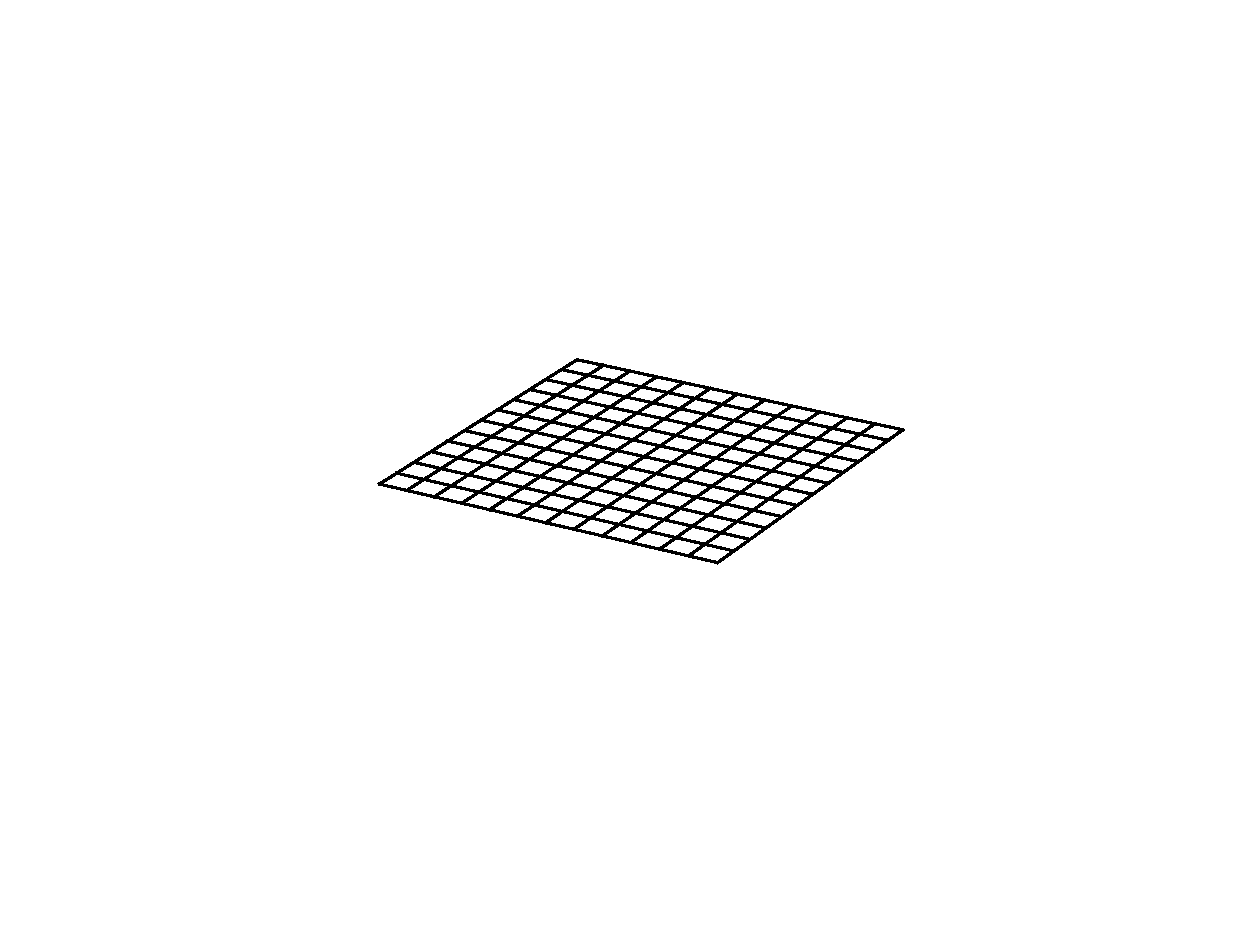
\includegraphics[trim=175 165 140 165, clip, scale=0.4]{../paper/FIG/tc1_platform}
                \end{figure}\end{textblock}
        }
        \only<2->{
            \begin{textblock}{7}(-1,1)\textbf{Problem:} find best antenna placements \end{textblock}
            \begin{textblock}{3}(2.5,1.2)
                \begin{figure}
                    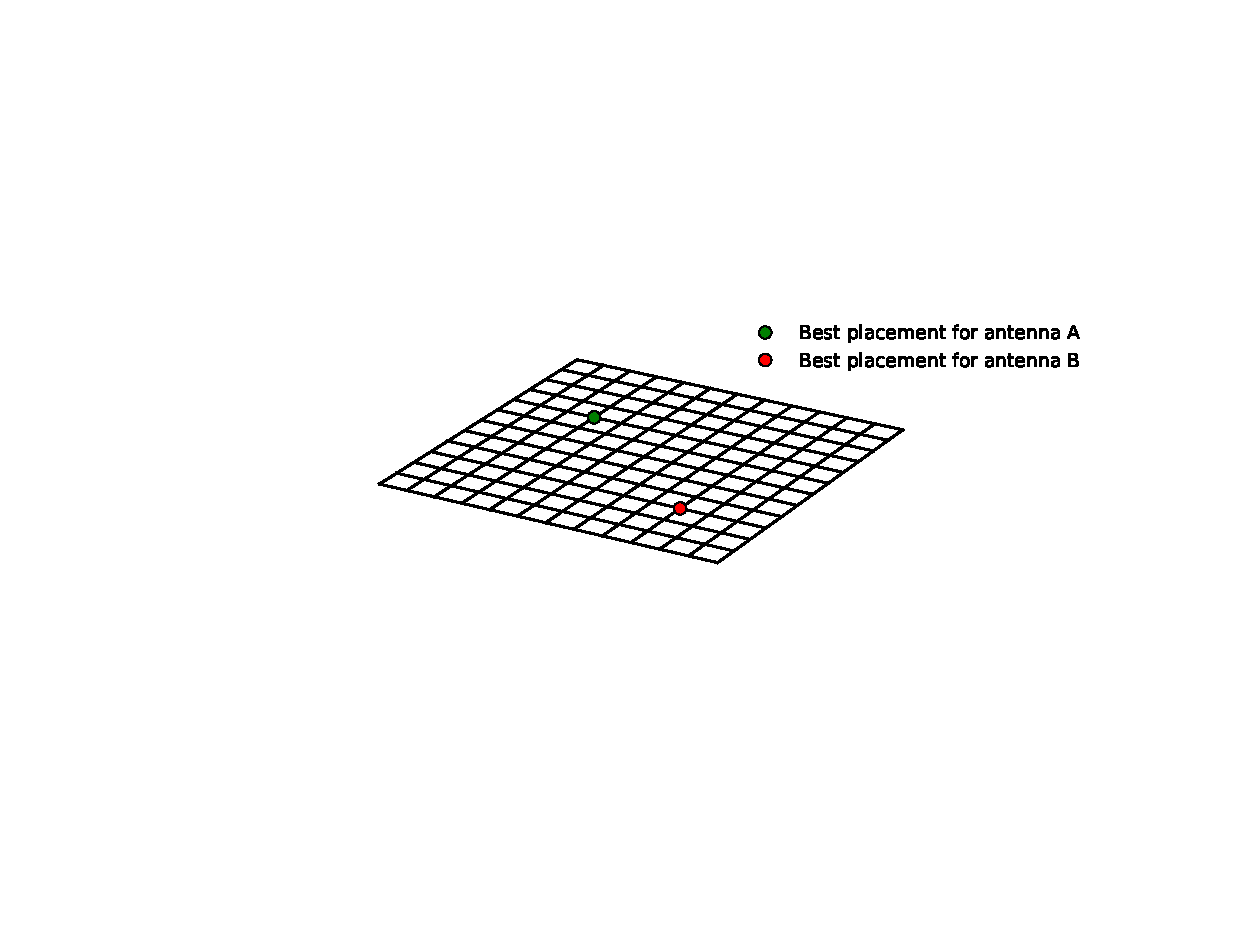
\includegraphics[trim=170 165 70 145, clip, scale=0.4]{../paper/FIG/tc11_intro}
                \end{figure}\end{textblock}
        }
        \column{0.33\linewidth}
        \only<1->{
            \begin{textblock}{6}(-1.5,-2.8) + \end{textblock}
            \begin{textblock}{6}(-0.7,-2.8) allowable placements of antennas \end{textblock}
            \begin{textblock}{3}(-0.2,-2)
                \begin{figure}
                    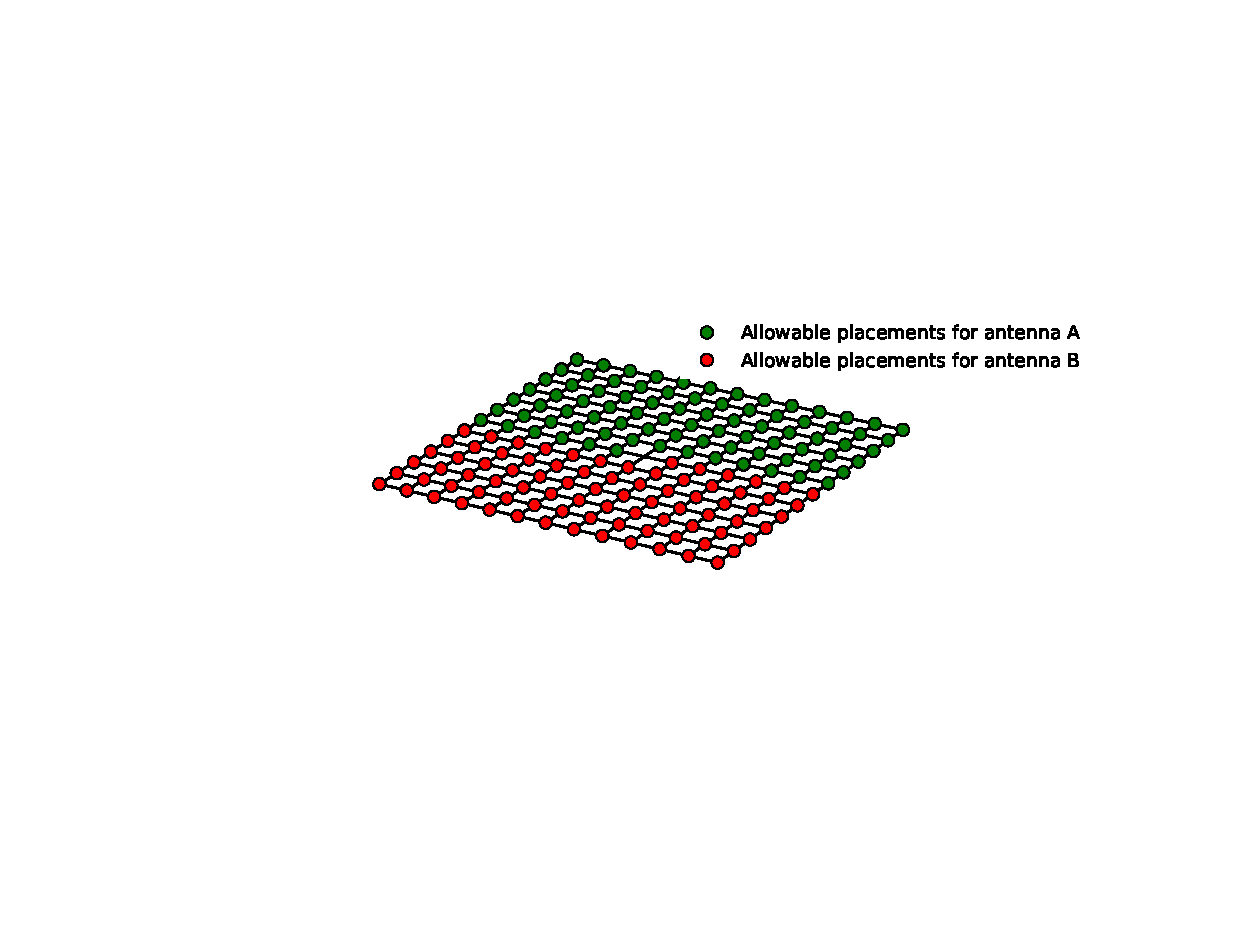
\includegraphics[trim=170 165 70 145, clip, scale=0.4]{../paper/FIG/tc1_intro}
                \end{figure}\end{textblock}
        }
    \end{columns}
\end{frame}

\begin{frame}[t]{Antenna Placement Problem}
    Given:
\begin{itemize} \itemsep1.5em
        \item platform $P$ with its surface gridded such that end points represent possible antenna placements
        \item set of  $m$ antennas $A = {A_1, A_2, \dots, A_m}$ such that $m > 1$
        \item for each $A_i$, $L_i$ denote the set of allowable placements $\in \mathbb R^3$ such that $\mid L_i \mid = n_i$ and $\forall i, n_i > 1$; $L_i = \{(x_{1}, y_{1}, z_{1}) \dots (x_{n_i}, y_{n_i}, z_{n_i})\}$
    \end{itemize}
    \vspace{10px}
    \centering\only{\textbf{Problem}: Find a set of $n$ optimal antenna placements on $P$}
\end{frame}

\begin{frame}{\null}
    \begin{tcolorbox}[colback=green!5]
        \centering
        Question: How is a good antenna placement quantified in the context of platform and other antennas?
    \end{tcolorbox}
\end{frame}

\begin{frame}[t]{Mutual Coupling}
    When two antennas are in proximity, and one is transmitting, the second will receive some of the transmitted energy.\\ \vspace{2mm}
    \begin{figure}\centering
        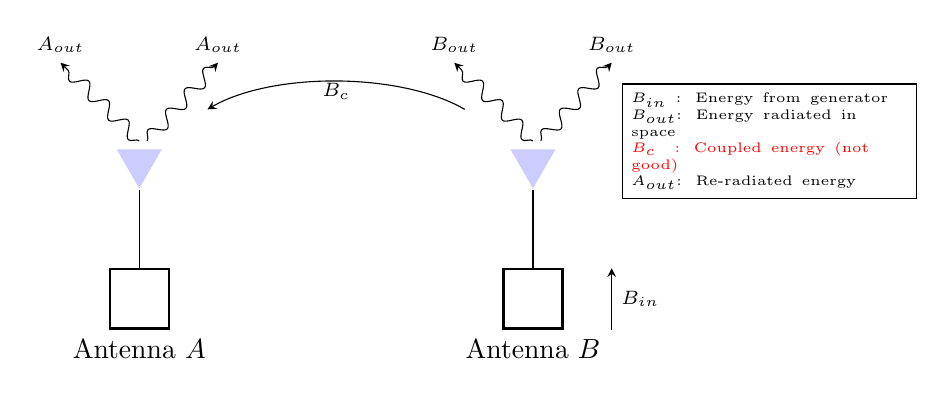
\begin{tikzpicture} [
                triangle/.style = {fill=blue!20, regular polygon, regular polygon sides=3 },
                node rotated/.style = {rotate=180},
                border rotated/.style = {shape border rotate=180}
            ]
            \node (b1) at (0, 1) [draw,thick,minimum width=.75cm,minimum height=.75cm, label=below:Antenna $A$] {}; 
            \node[triangle, border rotated, above=1cm of b1] (a1) {};
            \draw [-] (a1) -- (b1);
            \node (b2) at (5, 1) [draw,thick,minimum width=.75cm,minimum height=.75cm, label=below:Antenna $B$] {}; 
            \node[triangle, border rotated, above=1cm of b2] (a2) {};
            \draw [-] (a2) -- (b2);
            \draw [-stealth] ([xshift=1cm] b2.south) to node[right] {\scriptsize $B_{in}$} ([xshift=1cm] b2.north);
            \draw [stealth-, shorten <= 1cm, shorten >= 1cm] (a1.north) to[bend left] node {\scriptsize $B_c$} (a2.north);
            \draw [-stealth,decorate,decoration=snake] ([yshift=.1cm, xshift=.1cm] a1.north) -- (1,4) node[above] {\scriptsize $A_{out}$};
            \draw [-stealth,decorate,decoration=snake] ([yshift=.1cm] a1.north) -- (-1,4) node[above] {\scriptsize $A_{out}$};
            \draw [-stealth,decorate,decoration=snake] ([yshift=.1cm, xshift=.1cm] a2.north) -- (6,4) node[above] {\scriptsize $B_{out}$};
            \draw [-stealth,decorate,decoration=snake] ([yshift=.1cm] a2.north) -- (4,4) node[above] {\scriptsize $B_{out}$};
            \node[draw, text width=3.5cm] at (8,3) {\tiny $B_{in}~$:  Energy from generator\\$B_{out}$: Energy radiated in space\\{\color{red}$B_c~~$: Coupled energy (not good)}\\$A_{out}$: Re-radiated energy\\}; 
        \end{tikzpicture}
    \end{figure}
\end{frame}

\begin{frame}{Minimize Mutual Coupling}
    \begin{tcolorbox}[colback=green!5]
        \begin{equation}
            F_{MC} = \sum_{i=1}^{n-1}\sum_{j=i+1}^{n} CP(A_i, A_j),
        \end{equation}
    \end{tcolorbox}
    where
    \begin{itemize}
        \item $CP(\cdot, \cdot) \in \mathbb R$ is the coupling between two antennas, and computed using a simulator
    \end{itemize}
    \vspace{2mm}
    \small\textit{Example:} If $n=3$, then $F_{MC} = CP(A_1, A_2) + CP(A_1, A_3) + CP(A_2, A_3)$
\end{frame}


\begin{frame}{Minimize Difference in Radiation Pattern}
    Pattern defines the ratio of energy radiated and input energy in a particular direction. For each antenna $A_i$:
    \begin{tcolorbox}[colback=green!5]
        \begin{equation} \label{eq:rp}
            F_{RP} = \sum_{i=1}^n\sum_{\theta=0}^\pi\sum_{\phi=0}^{2\pi}
            \left( FSG_i(\theta,\phi) - ISG_i(\theta,\phi) \right) ^2,
        \end{equation}
    \end{tcolorbox}
    where
    \begin{itemize}
            \small
        \item $\theta, \phi$ spherical coordinates
        \item $FSG(\cdot)$ returns free-space gain pattern  
        \item $ISG(\cdot)$ returns in-situ gain pattern
    \end{itemize}

\end{frame}

\begin{frame}{Objective Function}
    Find a placement such that $F$ is minimal:
    \begin{tcolorbox}[colback=green!5]
        \begin{equation} \label{eq:optimal}
            F = \alpha F_{MC} + \beta F_{RP},
        \end{equation}
    \end{tcolorbox}
    where $\alpha, \beta$ are weights for each of the objectives 
\end{frame}

\begin{frame}{\null}
    \begin{tcolorbox}[colback=green!5]
        \centering\Huge
        Part 2: Stochastic Algorithms
    \end{tcolorbox}
\end{frame}

\begin{frame}[t]{Stochastic Algorithms}
    We will consider algorithms which rely on \textit{randomization} principle.
    \vspace{10px}
\begin{itemize} \itemsep1.5em
        \item Genetic Algorithm
        \item Evolutionary Strategy
        \item Simulated Annealing
        \item Hill Climbing
    \end{itemize}
    \vspace{5mm}
    Each algorithm maintains a candidate solution or pool of candidate solutions called population
\end{frame}

\begin{frame}[t]{Candidate Solution}
    Also referred as an \textbf{individual}
\begin{itemize} \itemsep1.5em
        \item Pool of individuals
            \adjustbox{valign=t}{%
                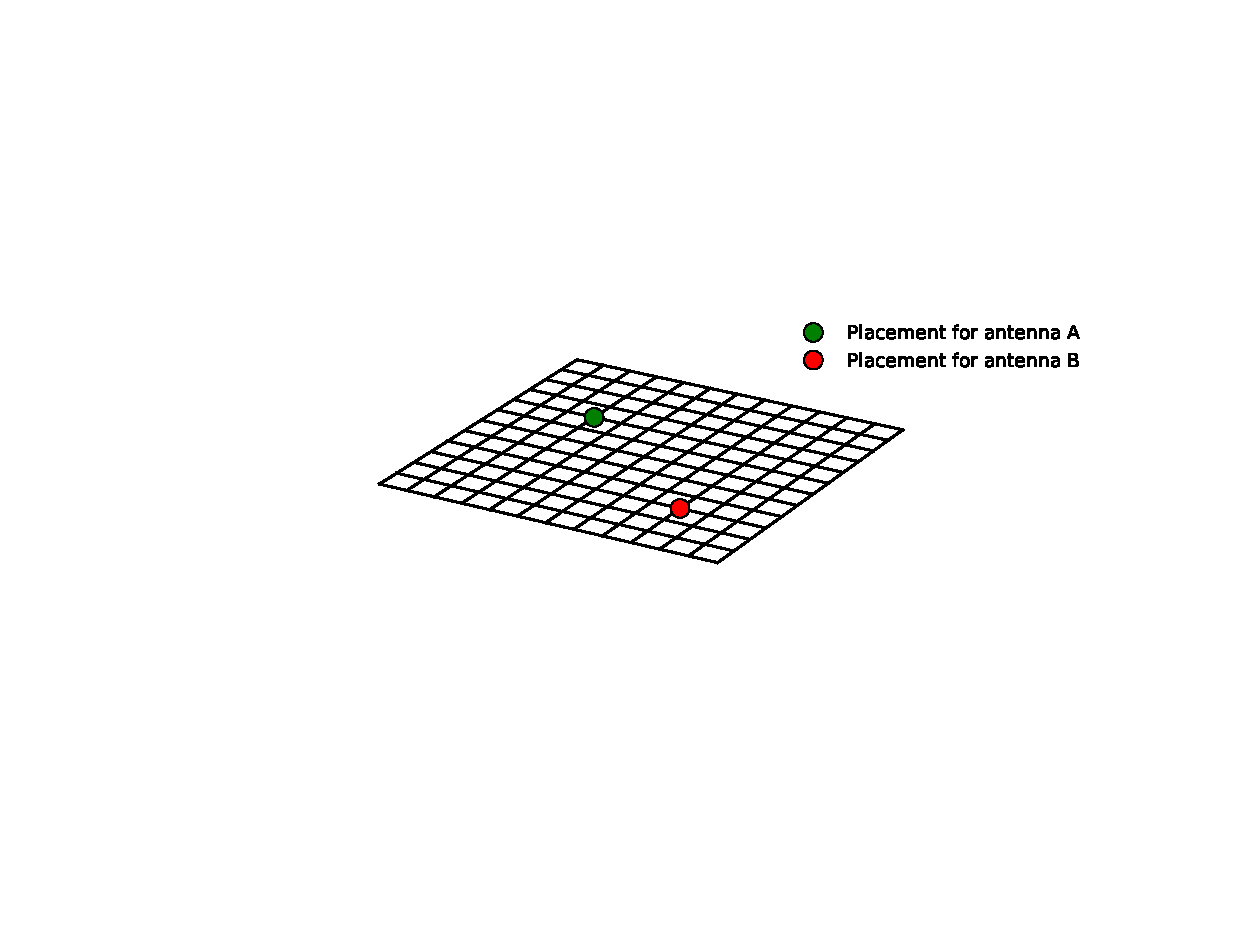
\includegraphics[trim=175 165 50 135, clip, scale=0.35]{../paper/FIG/tc1_mut1}
                $\bigcdot~\bigcdot~\bigcdot$
                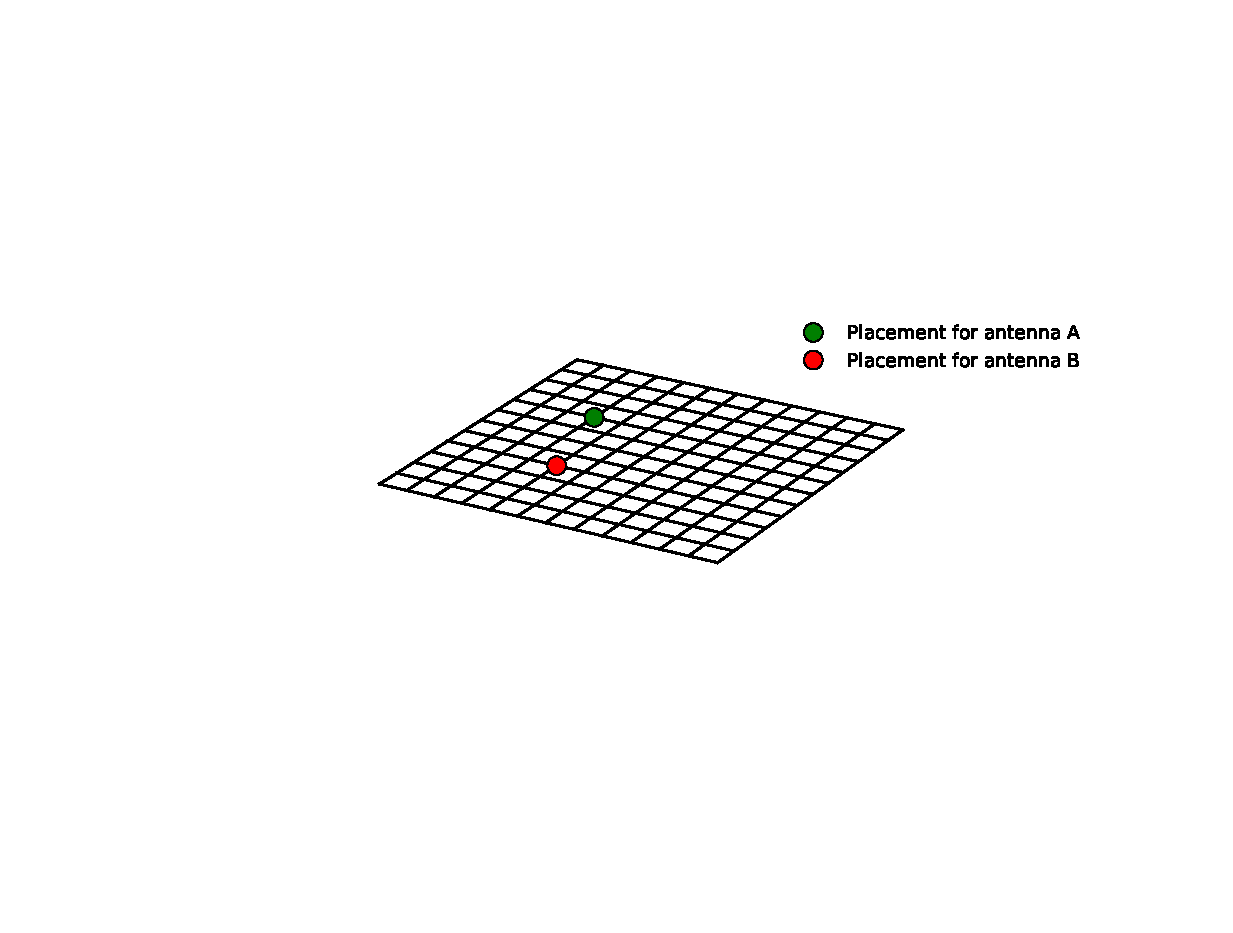
\includegraphics[trim=125 165 50 135, clip, scale=0.35]{../paper/FIG/tc1_mut3}
            }
        \item Single individual\\
            \adjustbox{valign=t}{%
                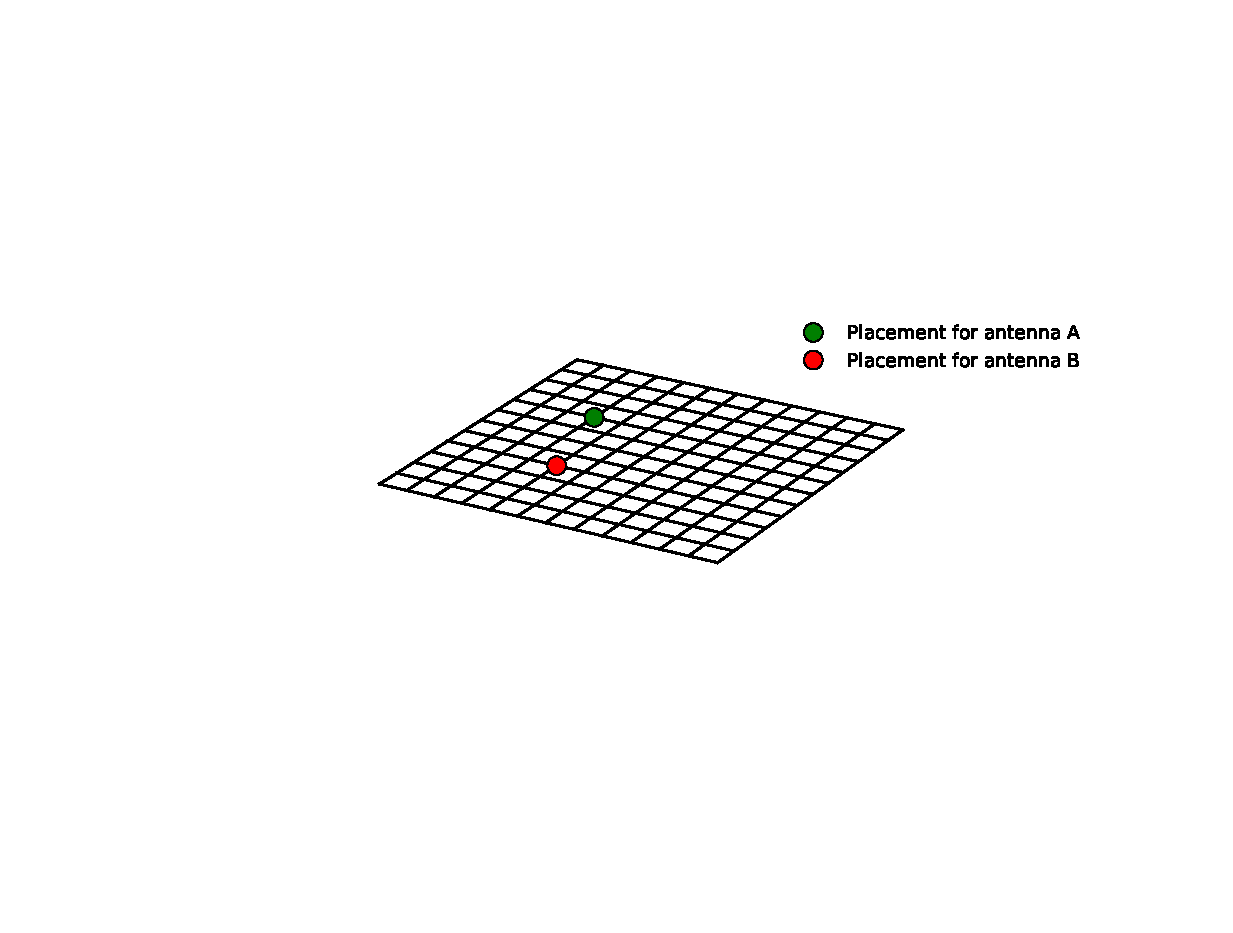
\includegraphics[trim=125 165 50 135, clip, scale=0.35]{../paper/FIG/tc1_mut3}
            }
    \end{itemize}
\end{frame}

\begin{frame}[t]{Stochastic Algorithms: Mutation Operator}
    \begin{enumerate}
        \item Given an individual, select an antenna uniformly at random, let's say antenna 1:\par
            \begin{minipage}[t]{\linewidth}
                \centering
                \adjustbox{valign=t}{%
                    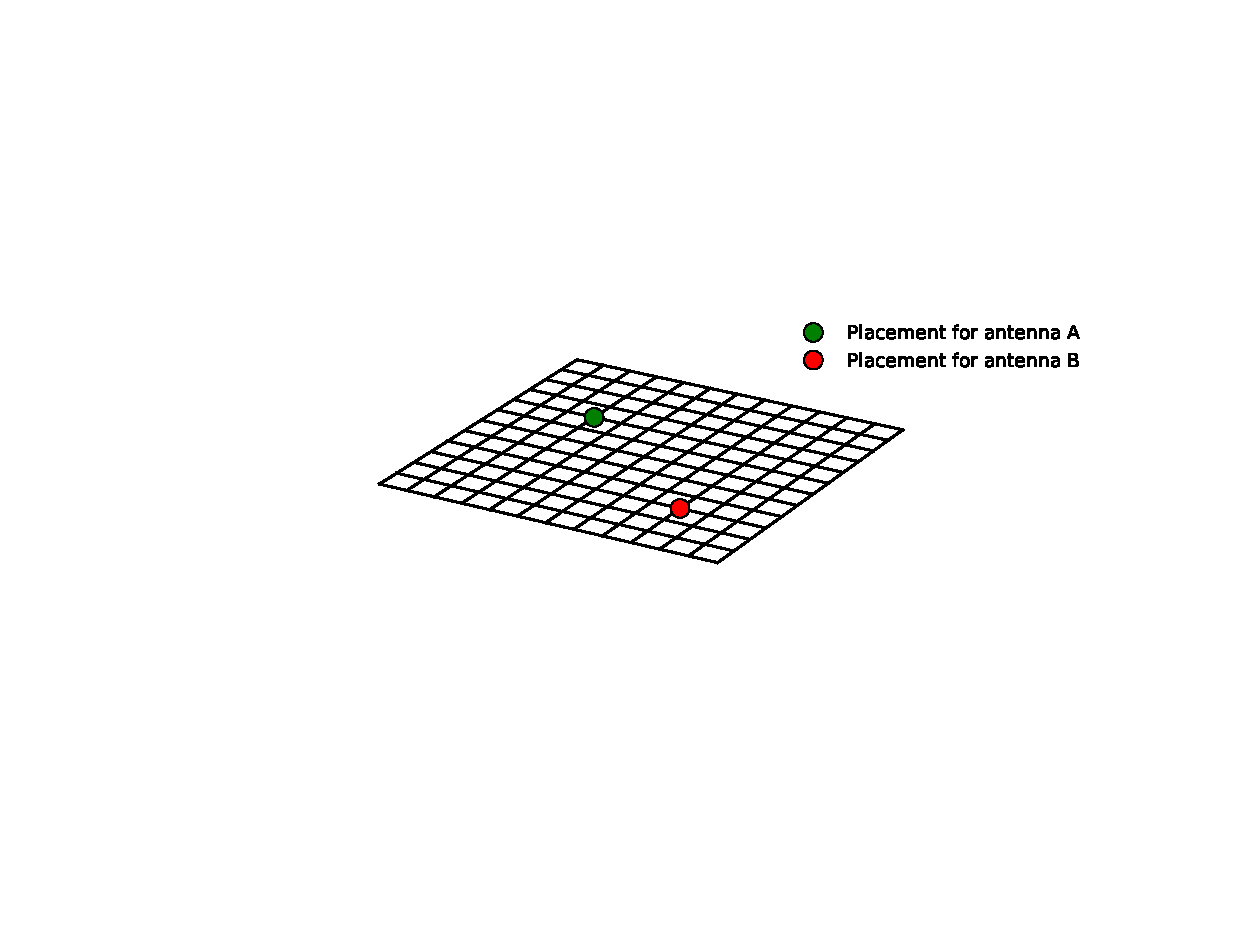
\includegraphics[trim=175 165 50 135, clip, scale=0.35]{../paper/FIG/tc1_mut1}
                }
            \end{minipage}
        \item For antenna 1, select any other placement:\par
            \begin{minipage}[t]{\linewidth}
                \centering
                \adjustbox{valign=t}{%
                    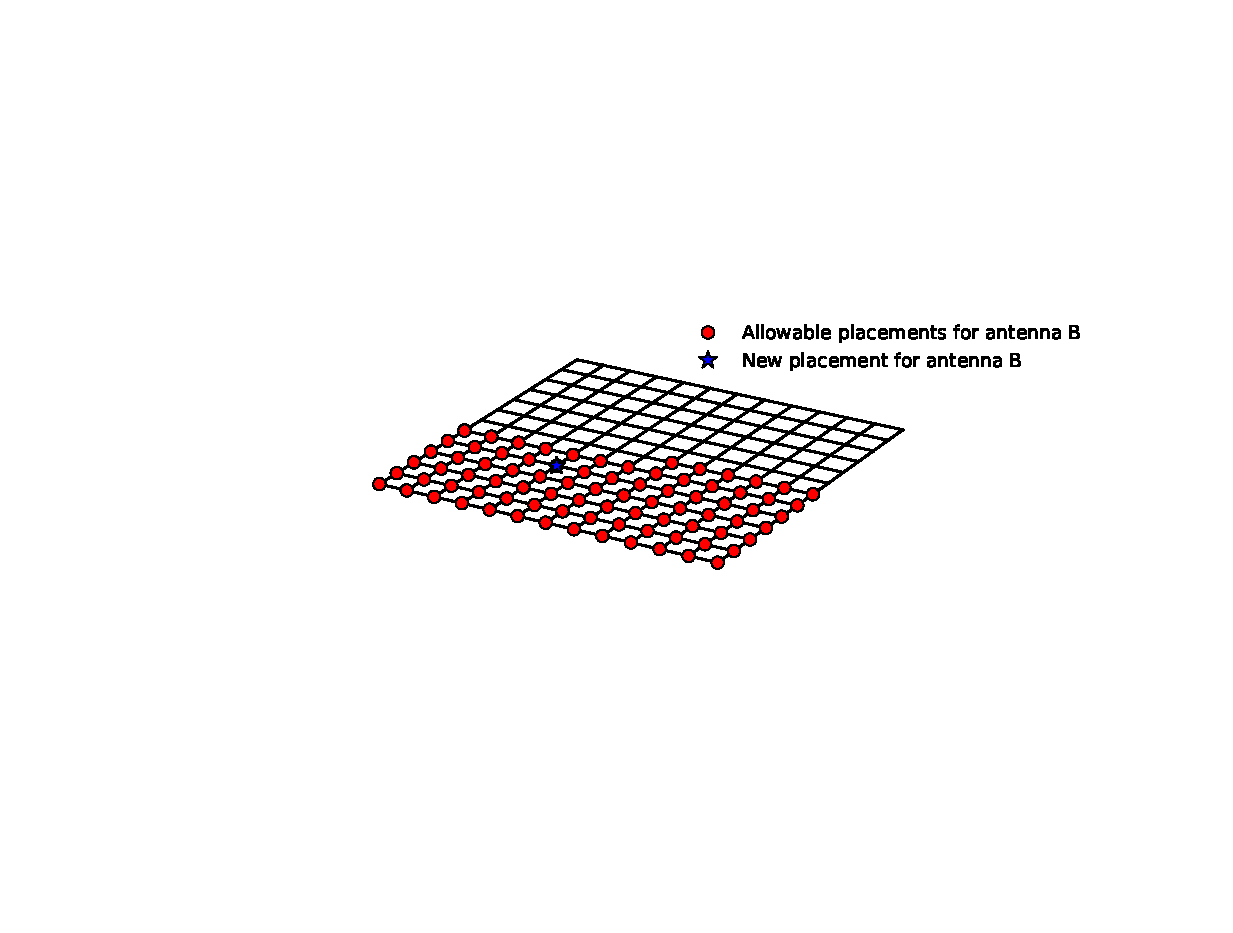
\includegraphics[trim=125 165 50 135, clip, scale=0.35]{../paper/FIG/tc1_mut2}
                }
            \end{minipage}
        \item Change position for antenna 1 in individual:\par
            \begin{minipage}[t]{\linewidth}
                \centering
                \adjustbox{valign=t}{%
                    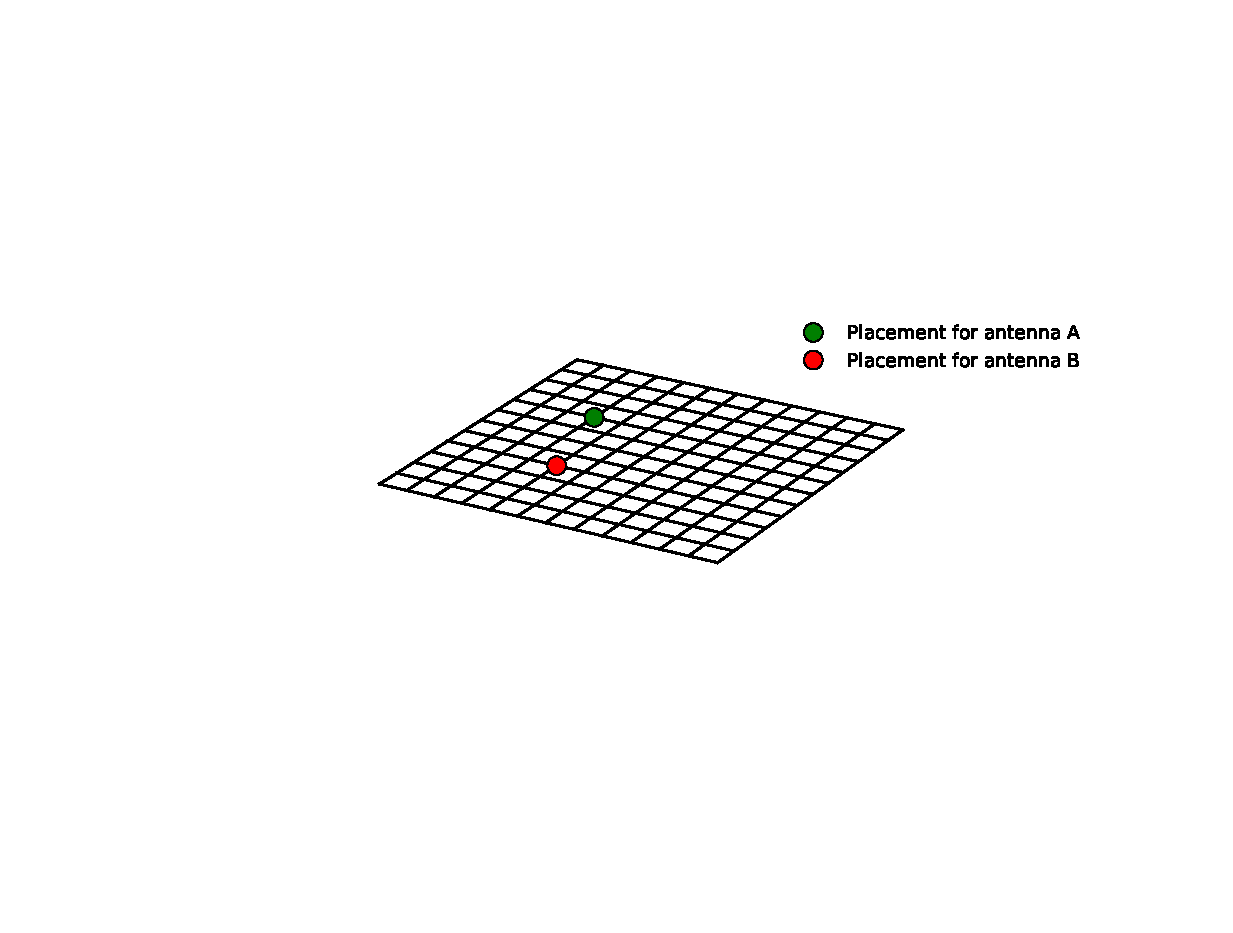
\includegraphics[trim=125 165 50 135, clip, scale=0.35]{../paper/FIG/tc1_mut3}
                }
            \end{minipage}
    \end{enumerate}
\end{frame}

\begin{frame}[t]{Stochastic Algorithms: Crossover Operator}
    \begin{enumerate}
        \item Select two individuals from population:\par
            \begin{minipage}[t]{\linewidth}
                \centering
                \adjustbox{valign=t}{%
                    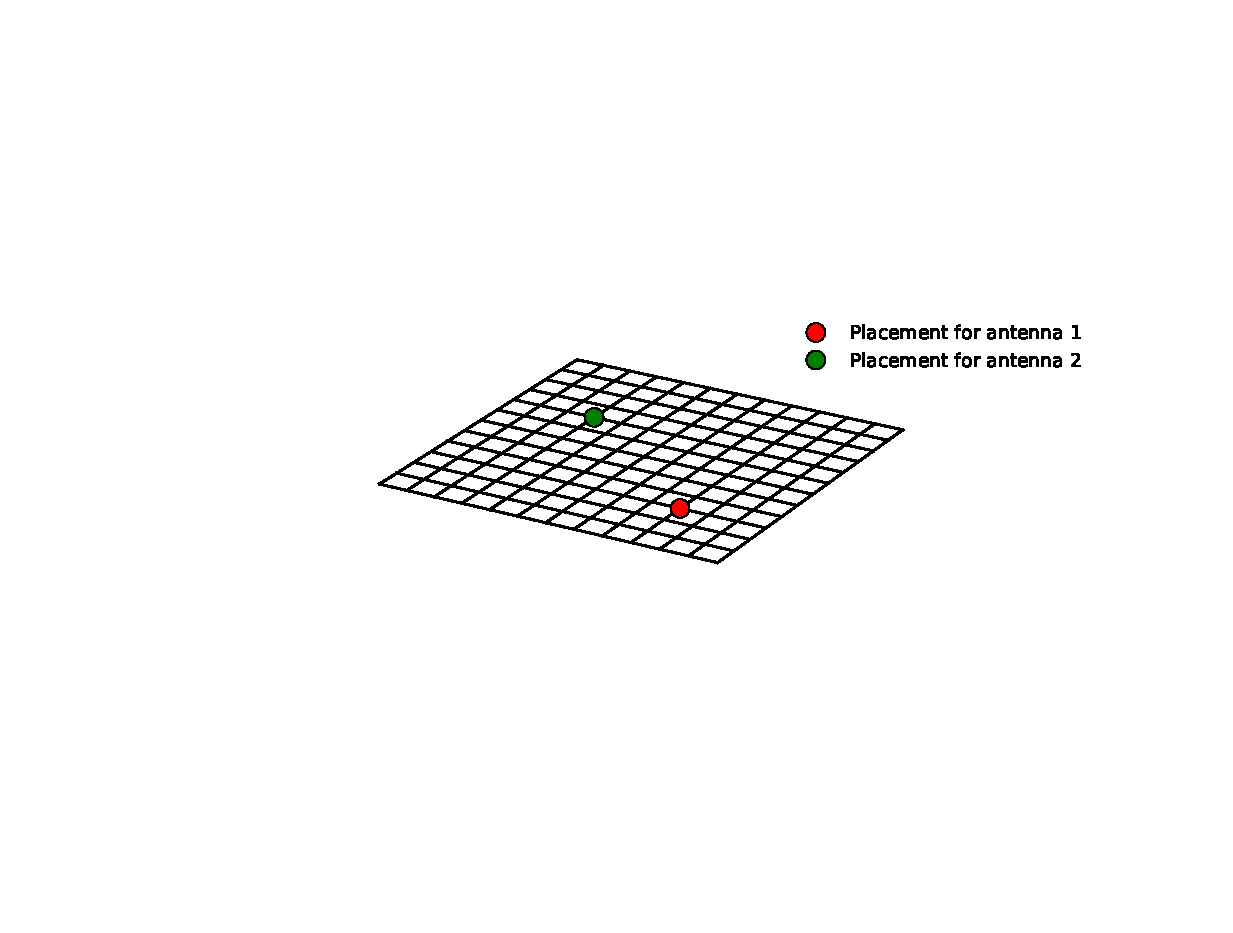
\includegraphics[trim=175 165 50 135, clip, scale=0.35]{../paper/FIG/tc1_reco1}
                    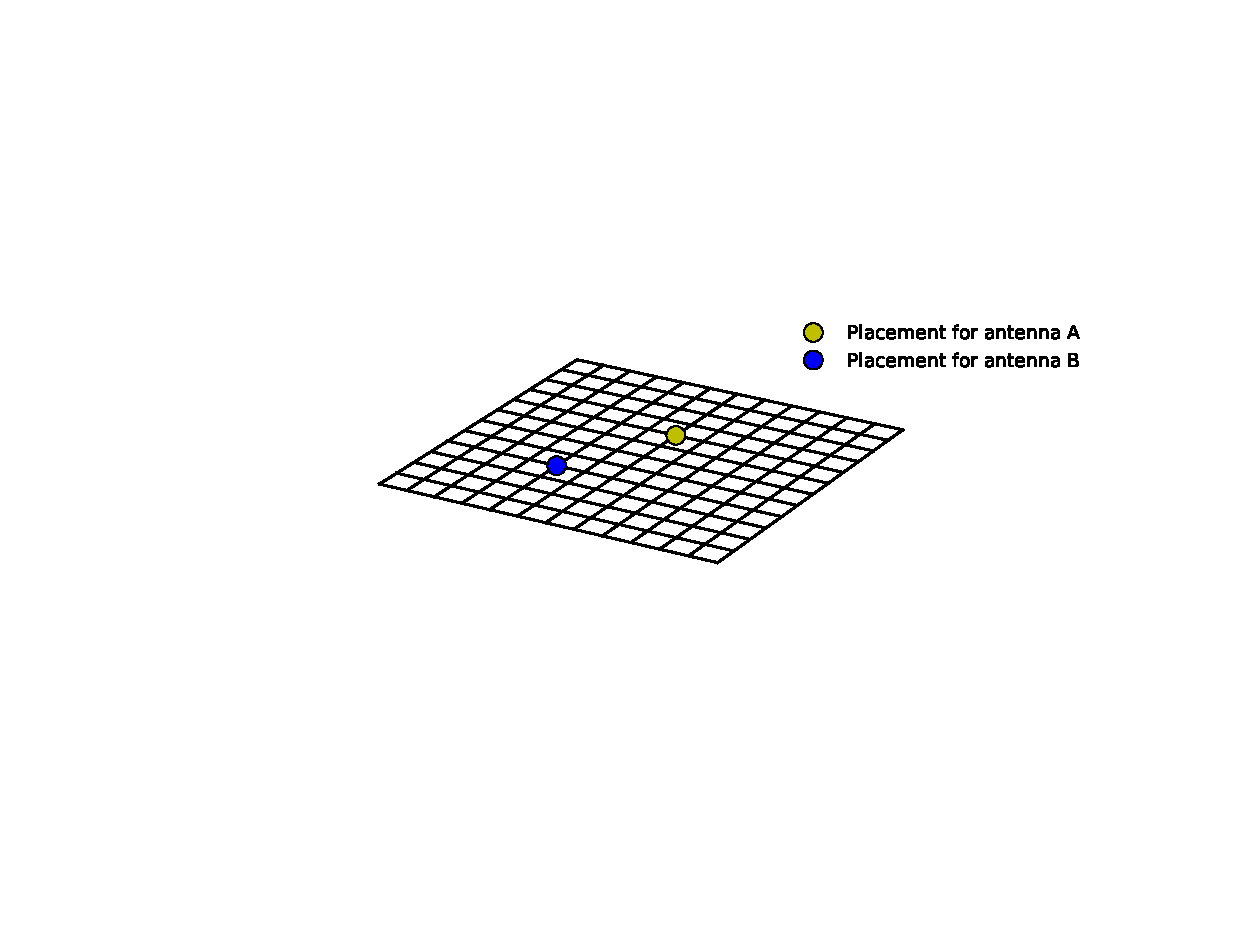
\includegraphics[trim=175 165 50 135, clip, scale=0.35]{../paper/FIG/tc1_reco2}
                }
            \end{minipage}
        \item Select a crossover point, and swap placements prior to the point: \par
            \begin{minipage}[t]{\linewidth}
                \centering
                \adjustbox{valign=t}{%
                    \begin{tabular}{ll:l}
                        $\text{ind}_1:$&$\textcolor{red}{A_1}$ & $\textcolor{drkgreen}{A_2}$ \\
                        &\makebox[\widthof{A\_1}][l]{$\downarrow~\uparrow$} &\\
                        $\text{ind}_2:$&$\textcolor{blue}{A_1}$ & $\textcolor{aureolin}{A_2}$ \\
                    \end{tabular}
                }
            \end{minipage}
        \item Two new offsprings created:\par
            \begin{minipage}[t]{\linewidth}
                \centering
                \adjustbox{valign=t}{%
                    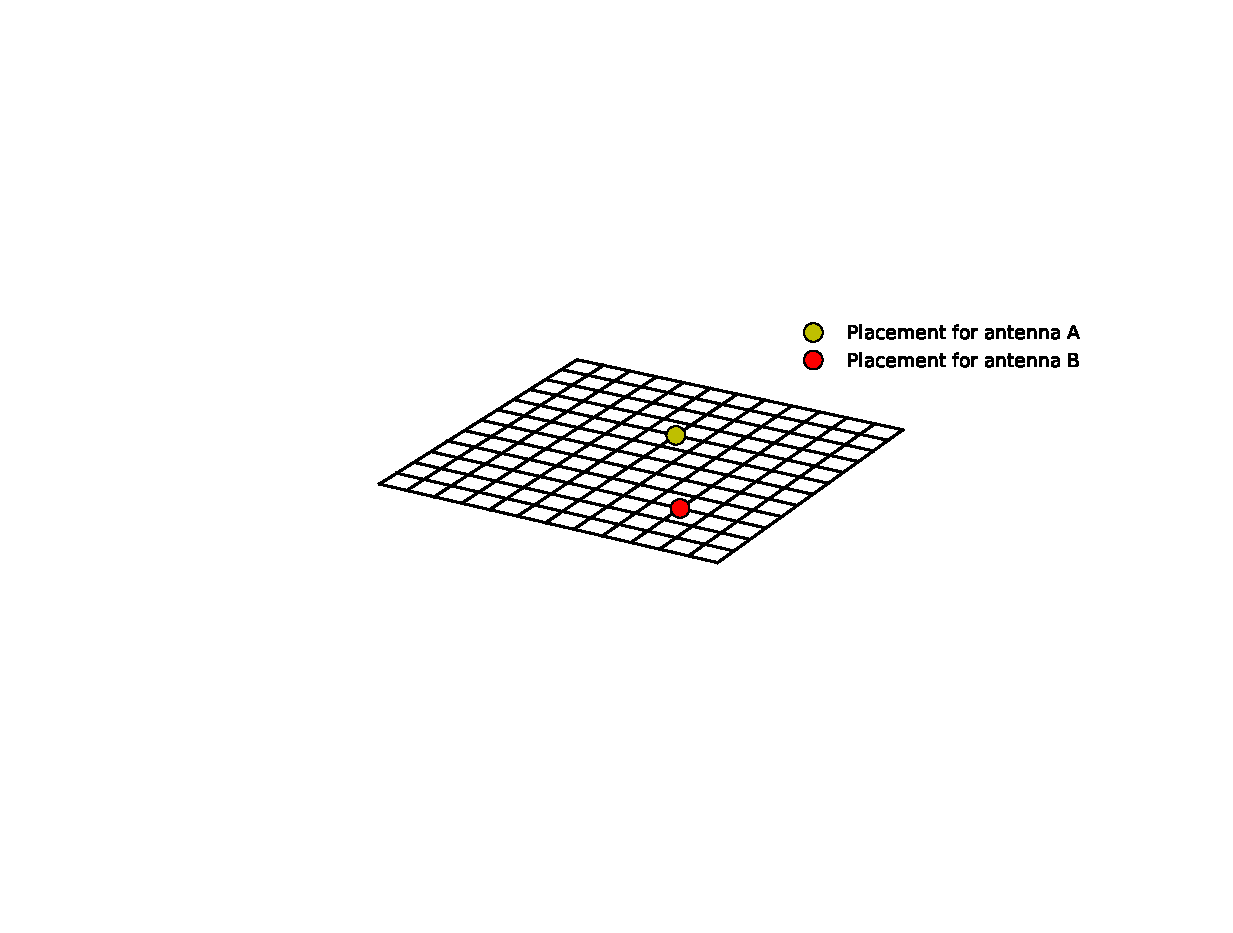
\includegraphics[trim=175 165 50 135, clip, scale=0.35]{../paper/FIG/tc1_reco3}
                    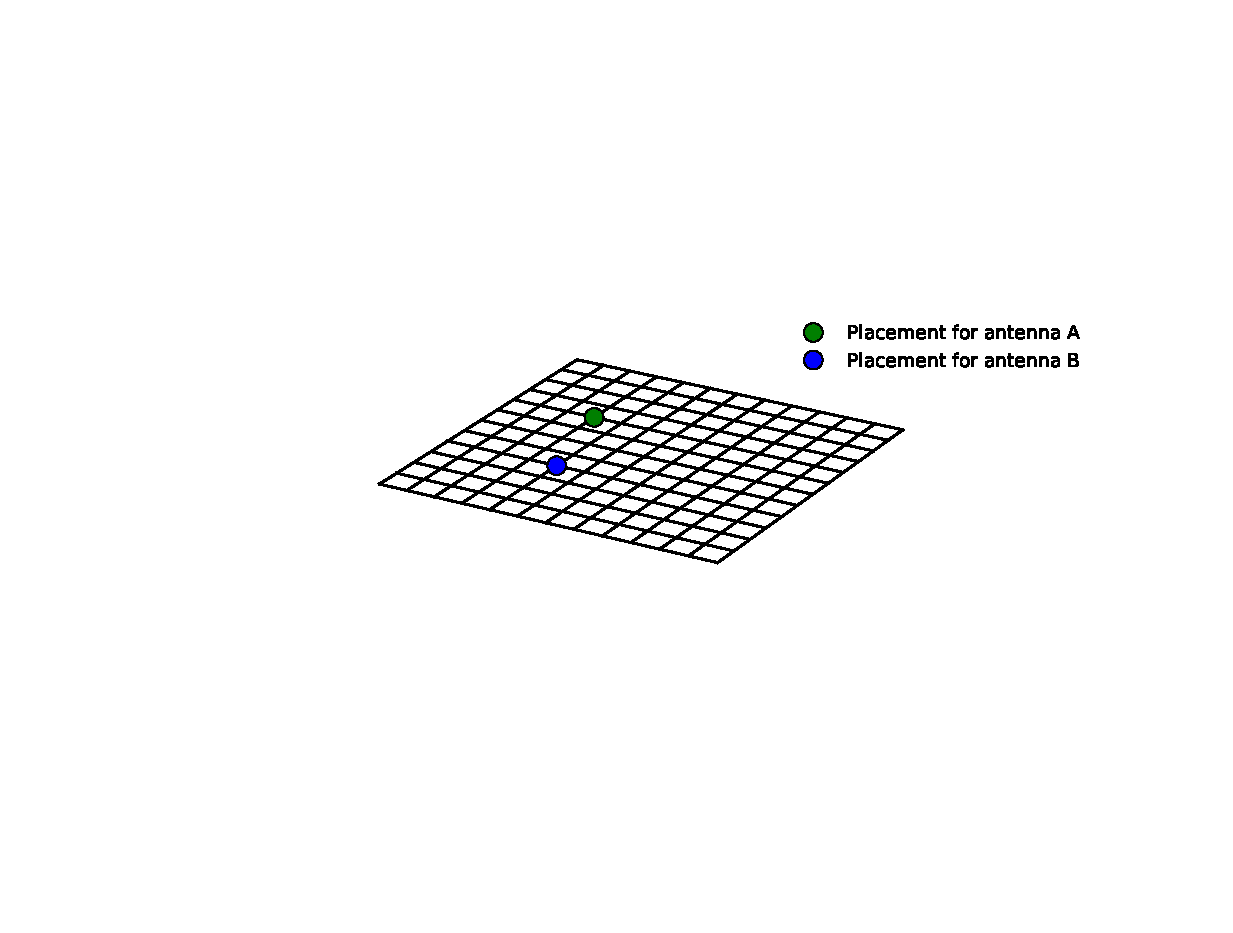
\includegraphics[trim=175 165 50 135, clip, scale=0.35]{../paper/FIG/tc1_reco4}
                }
            \end{minipage}
    \end{enumerate}
\end{frame}

\begin{frame}{\null}
    \begin{tcolorbox}[colback=green!5]
        \centering
        Question: Why use stochastic algorithms?
    \end{tcolorbox}
\end{frame}

\begin{frame}[t]{Multi-Modal Search Space}
    \begin{figure}
        \vspace*{-0.35cm}
        \centering
        \includegraphics[scale=0.48]{../paper/FIG/tc1_ss}
    \end{figure}
\end{frame}

\begin{frame}{Genetic Algorithm}
    \begin{columns}
        \begin{column}{0.66\linewidth}%added for this algorithm since text wasn't fitting in one slide
            \begin{spacing}{0.6}
                \fontsize{8}{12}\selectfont
                \setlength{\interspacetitleruled}{0pt}%
                \setlength{\algotitleheightrule}{0pt}%
                \begin{algorithm}[H]
                    \only<1>{\highlight{\textbf{P} $\leftarrow$ generate $p$ random individuals. Compute $fitness(ind_i), i \in [1,p]$}\;}
                    \only<2>{\textbf{P} $\leftarrow$ generate $p$ random individuals. Compute $fitness(ind_i), i \in [1,p]$\;}
                    $i=0$ \;
                    \While{$i<gen_{max}$} {
                        \only<1>{Elitism: Select $n_e$ fittest individuals to add to \textbf{P'}} \;
                        \only<2>{\highlight{Elitism: Select $n_e$ fittest individuals to add to \textbf{P'}} \;}
                        \For{$(p - n_e)/2$ times} {
                            \tcc{select returns pair of individuals}
                            $\textbf{M} \leftarrow select(\textbf{P}, 2)$  \;
                            \eIf {$rand(0,1)<p_c$} {
                                \only<1>{Apply $crossover(M)$ to get two offsprings \textbf{O} \;}
                                \only<2>{\highlight{Apply $crossover(M)$ to get two offsprings \textbf{O}} \;}
                                Add $O$ to $P'$ \;
                            }
                            { Add $M$ to $P'$ \; }
                        }
                        \only<1>{Uniformly select $p_{m} \cdot (p - n_e)$ individuals from $P$, and apply $mutation$ operator to each \;}
                        \only<2>{\highlight{Uniformly select $p_{m} \cdot (p - n_e)$ individuals from $P$, and apply $mutation$ operator to each} \;}
                        Update $P\leftarrow P'$ \;
                        Compute $fitness(ind_i); i \in [1, p]$\;
                        Update $i \leftarrow i + 1$ \;
                    }
                \end{algorithm}
            \end{spacing}
        \end{column}
        \begin{column}{0.3\linewidth}
            \only<2->
            {
                \begin{figure}
                    \centerline{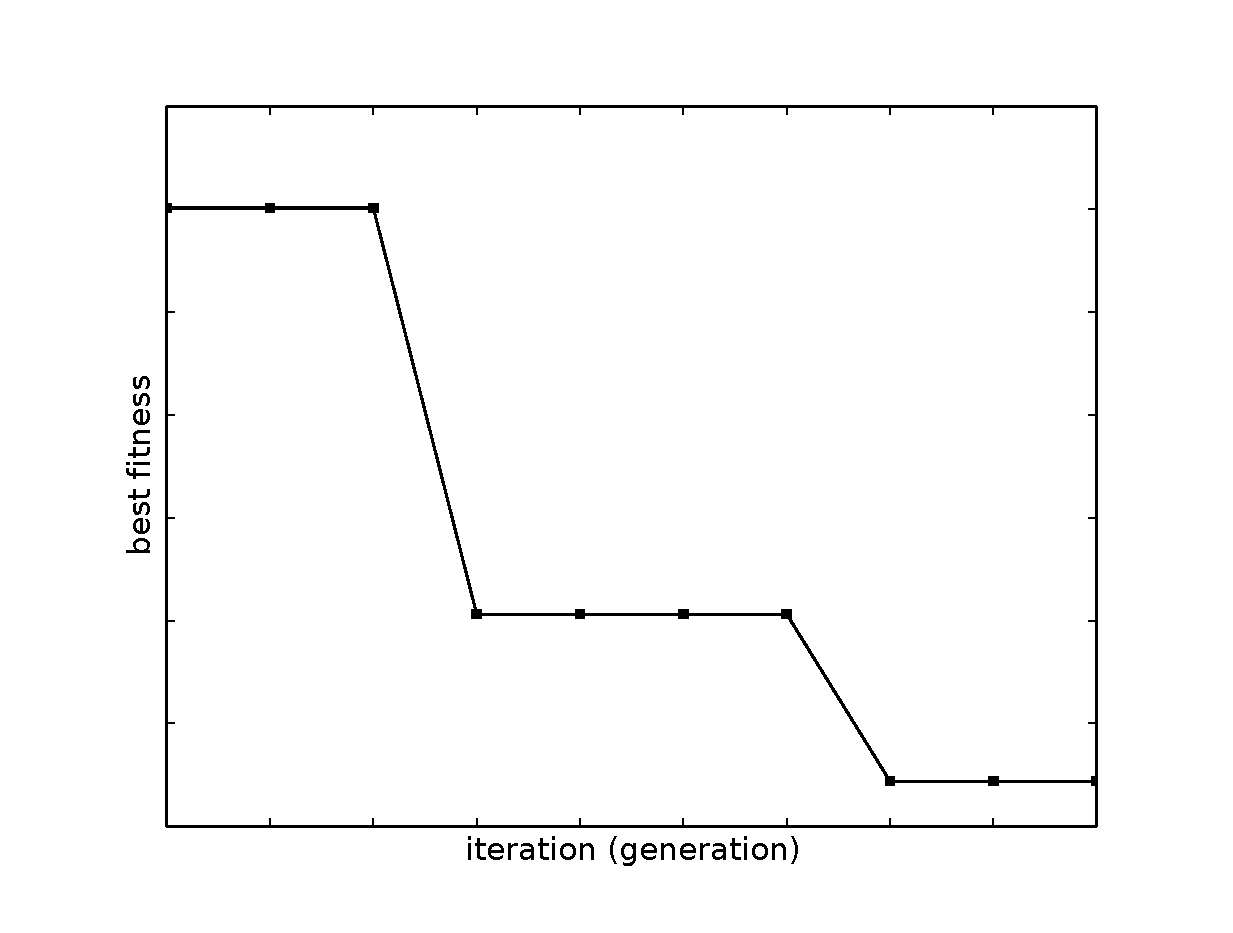
\includegraphics[width=5cm]{../paper/FIG/algo_ga}}
                    \caption*{\highlight{Plateaus suggesting stagnation of search}}
                \end{figure}
            }
        \end{column}
    \end{columns}
\end{frame}


\begin{frame}{Evolutionary Strategy}
    \begin{columns}
        \begin{column}{0.66\linewidth}
            \fontsize{8}{12}\selectfont
            \setlength{\interspacetitleruled}{0pt}%
            \setlength{\algotitleheightrule}{0pt}%
            \begin{algorithm}[H]
                \only<1>{\highlight{\textbf{P}$\leftarrow$ generate $\mu$ random individuals} \;}
                \only<2>{\textbf{P}$\leftarrow$ generate $\mu$ random individuals \;}
                $i=0$ \;
                \While{$i<gen_{max}$} {
                    \only<1>{Create $\lambda / \mu$ offsprings from  each $\mu$ individuals by applying $mutation$ operator, and add all offsprings to \textbf{P}\;}
                    \only<2>{\highlight{Create $\lambda / \mu$ offsprings from  each $\mu$ individuals by applying $mutation$ operator, and add all offsprings to \textbf{P}} \;}
                    Compute $fitness(ind_i), i \in [1,\lambda]$ \;
                    \only<1>{Keep $\mu$ best individuals in \textbf{P}, and discard remaining $\lambda - \mu$ individuals \;}
                    \only<2>{\highlight{Keep $\mu$ best individuals in \textbf{P}, and discard remaining $\lambda - \mu$ individuals} \;}
                    Update $i \leftarrow i+1$
                }
            \end{algorithm}
        \end{column}
        \begin{column}{0.3\linewidth}
            \only<2->
            {
                \begin{figure}
                    \centerline{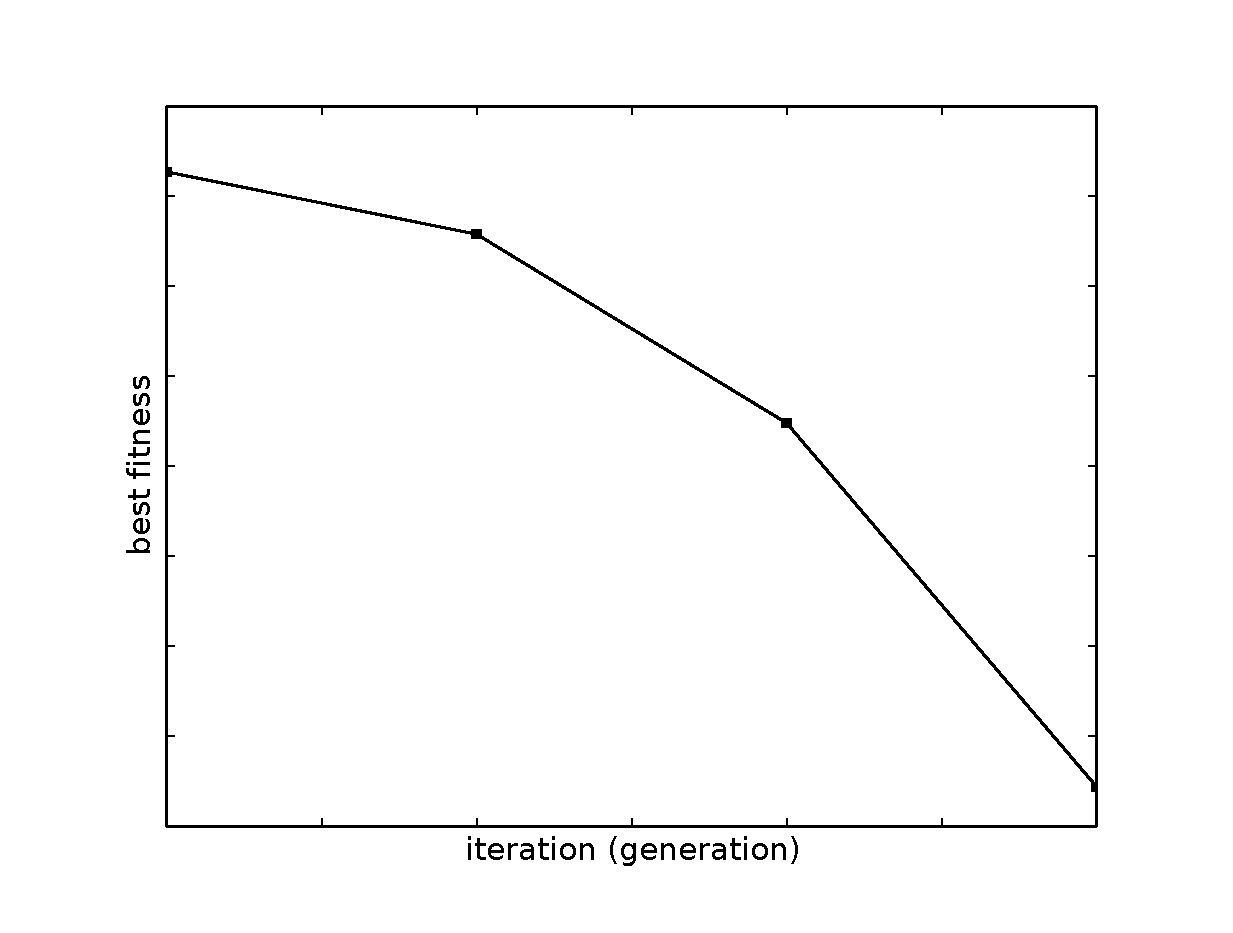
\includegraphics[width=5cm]{../paper/FIG/algo_es}}
                    \caption*{\highlight{No stagnation in exploration of search space}}
                \end{figure}
            }
        \end{column}
    \end{columns}
\end{frame}

\begin{frame}{Simulated Annealing}
    \begin{columns}
        \begin{column}{0.66\linewidth}
            \setlength{\interspacetitleruled}{0pt}%
            \setlength{\algotitleheightrule}{0pt}%
            \fontsize{8}{8}\selectfont
            \begin{algorithm}[H]
%\scriptsize
                \only<1>{\highlight{\textbf{c} $\leftarrow$ generate a random individual} \;}
                \only<2>{\textbf{c} $\leftarrow$ generate a random individual \;}
                $i=0$ \;
                \While{$i<i_max$} 
                {
                    \textbf{n} $\leftarrow mutate(\textbf{c})$ \; 
                    \eIf{$fitness(\textbf{c}) < fitness(\textbf{n})$} 
                    {
                        \If{\only<1>{$rand(0,1) < e^{-\delta f / T}$} \only<2>{\highlight{$rand(0,1) < e^{-\delta f / T}$}}} 
                        {
                            \only<1>{\textbf{c} $ \leftarrow $ \textbf{n}}
                            \only<2>{\highlight{\textbf{c} $ \leftarrow $ \textbf{n}}}
                        }
                    }  {$\textbf{c} \leftarrow \textbf{n}$ \; }
                    \only<1>{$T \leftarrow T \cdot f_{cooling}$ \;}
                    \only<2>{\highlight{$T \leftarrow T \cdot f_{cooling}$} \;}
                    $i \leftarrow i + 1$ \;
                } 
                \label{alg:ap-sa}
            \end{algorithm}
        \end{column}
        \begin{column}{0.3\linewidth}
            \only<2->
            {
                \begin{figure}
                    \centerline{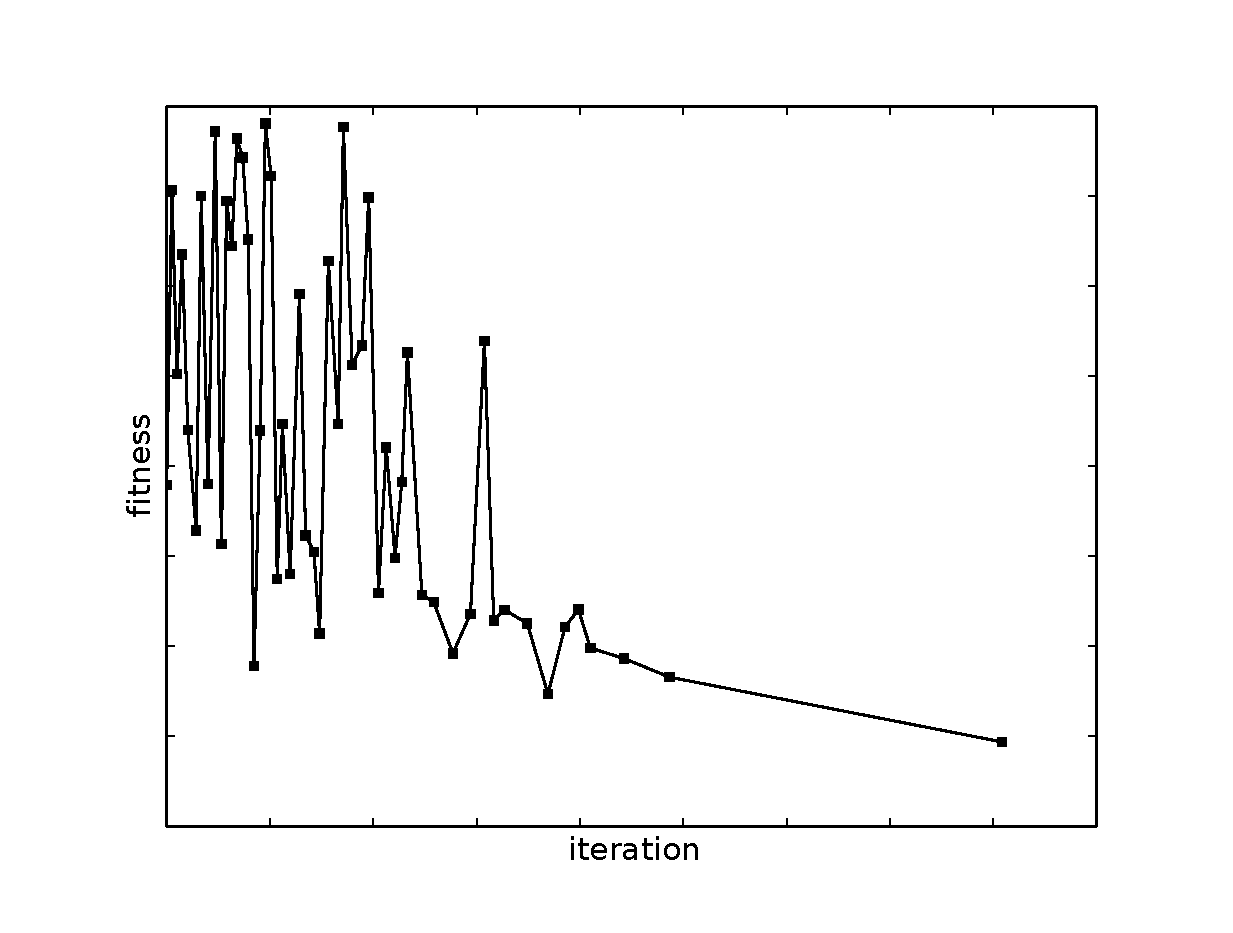
\includegraphics[width=5cm]{../paper/FIG/algo_sa}}
                    \caption*{\highlight{Fluctuation in fitness gradually reduces due to cooling}}
                \end{figure}
            }
        \end{column}
    \end{columns}
\end{frame}

\begin{frame}{Hill Climbing}
    \begin{columns}
        \begin{column}{0.66\linewidth}
            \setlength{\interspacetitleruled}{0pt}%
            \setlength{\algotitleheightrule}{0pt}%
            \fontsize{8}{8}\selectfont
            \begin{algorithm}[H]
                \only<1>{\highlight{Initialize \textbf{c} $\leftarrow$ generate a random inidividual} \;}
                \only<2>{Initialize \textbf{c} $\leftarrow$ generate a random inidividual \;}
                Compute $fitness(\textbf{c})$  \;
                $i=0$ \;
                \While{$i<i_{max}$} 
                {
                    \textbf{n} $\leftarrow mutate(\textbf{c})$ \; 
                    \If{\only<1>{$fitness(\textbf{n}) < fitness(\textbf{c})$} \only<2>{\highlight{$fitness(n) < fitness(c)$}}} 
                    {
                        \only<1>{$c \leftarrow n$} 
                        \only<2>{\highlight{$c \leftarrow n$}}
                    }
                    $i \leftarrow i + 1$
                }
                \label{alg:ap-hc}
            \end{algorithm}
        \end{column}
        \begin{column}{0.3\linewidth}
            \only<2->
            {
                \begin{figure}
                    \centerline{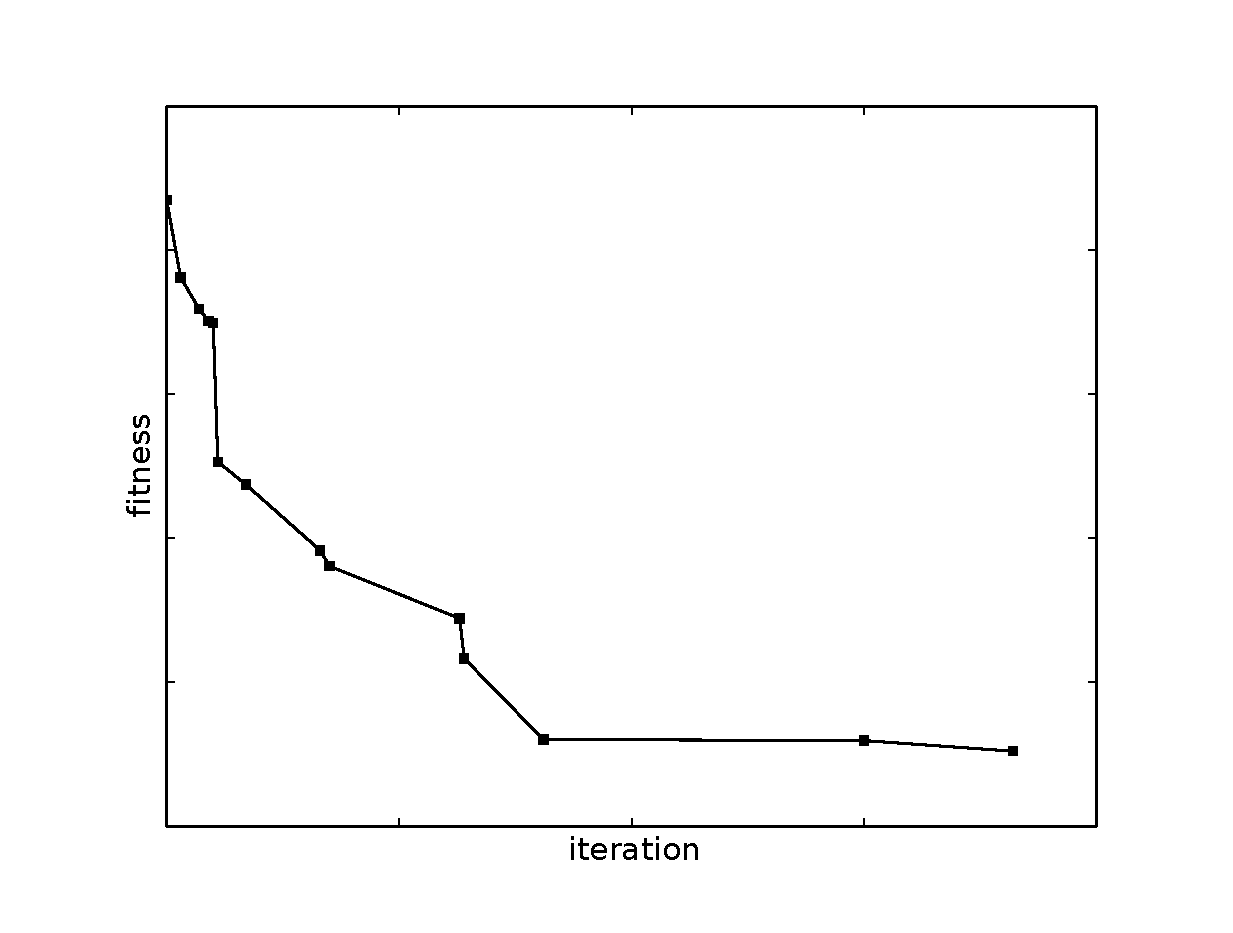
\includegraphics[width=5cm]{../paper/FIG/algo_hc}}
                    \caption*{\highlight{Only accepts fitter individual}}
                \end{figure}
            }
        \end{column}
    \end{columns}
\end{frame}

\begin{frame}{\null}
    \begin{tcolorbox}[colback=green!5]
        \centering\Huge
        Part 3: Results of real world experiments
    \end{tcolorbox}
\end{frame}

\begin{frame}[t]{Experimental Setup}
    \begin{enumerate}
        \item All test cases describe platforms which are replicas of real-world use cases like mobile devices, tanks, and cars
        \item We use a popular \textit{NEC2} simulator \footnote{http://www.nec2.org} to get fitness parameters 
        \item Evaluate the entire search space using an exhaustive algorithm to find the optimal antenna locations
    \end{enumerate}
    \vspace{10mm}
\end{frame}


\begin{frame}{Experiments: Test Cases}
    \begin{figure}
        \centering
        \begin{subfigure}{.5\columnwidth}
            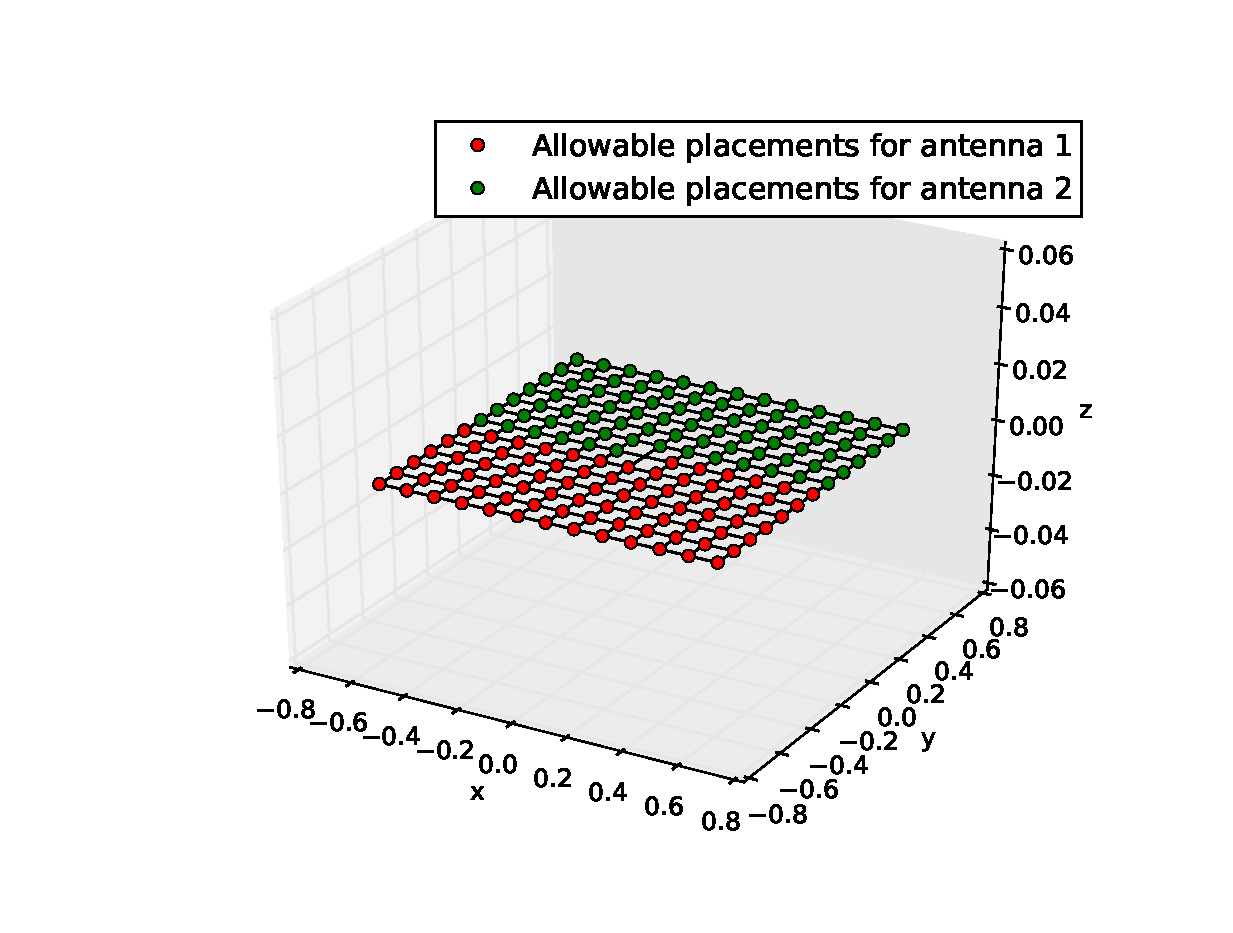
\includegraphics[width=\columnwidth,height=\columnwidth]{../paper/FIG/tc1_figure}%
            \caption*{\tiny Test Case \#1 with $7056 (84x84)$ allowable placements}%
        \end{subfigure}\hfill%
        \begin{subfigure}{.5\columnwidth}
            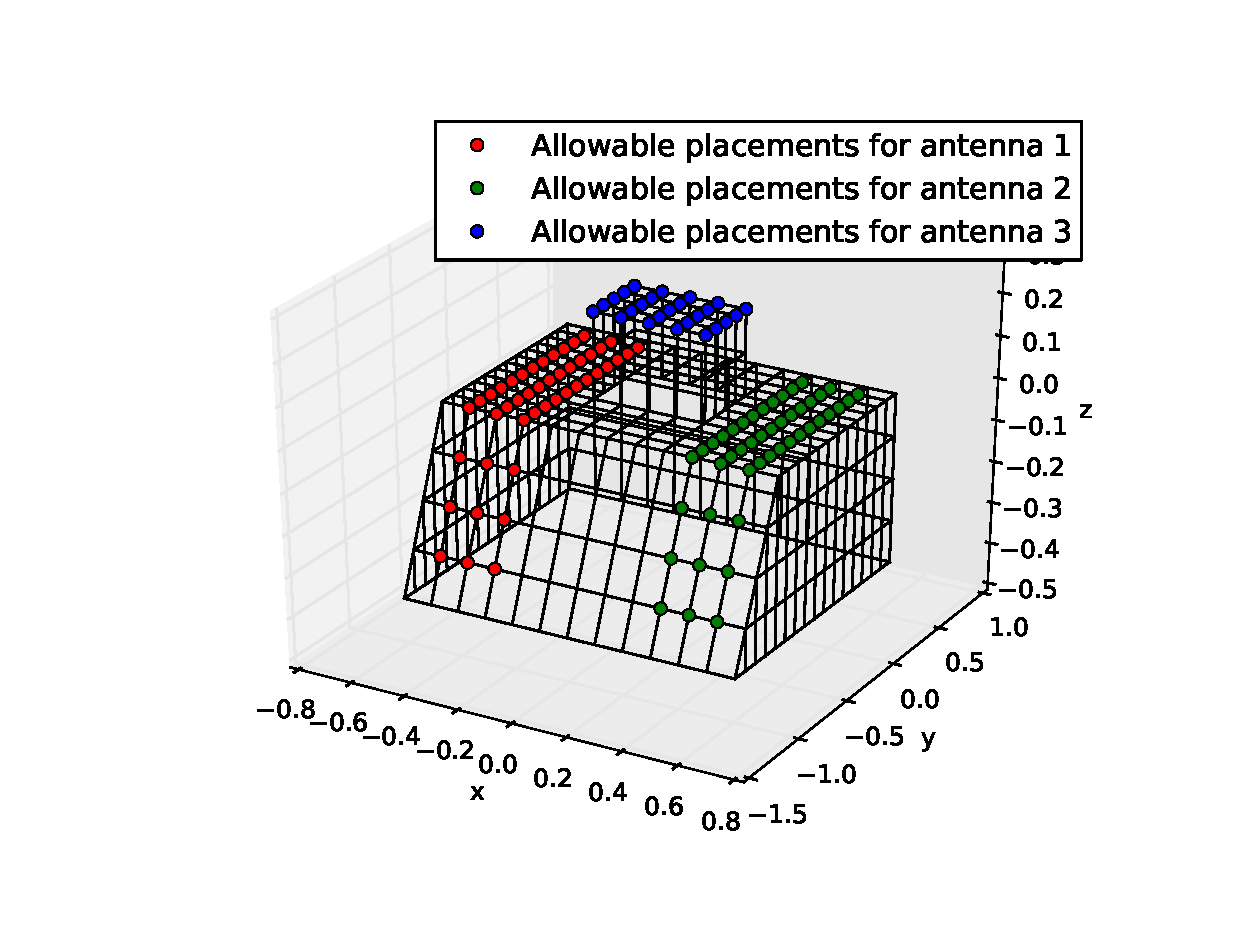
\includegraphics[width=\columnwidth, height=\columnwidth]{../paper/FIG/tc2_figure}%
            \caption*{\tiny Test Case \#2 with $50625 (45x45x45)$ allowable placements}%
        \end{subfigure}\hfill\\%
    \end{figure}
\end{frame}


\begin{frame}{Experiments: Test Cases}
    \begin{figure}
        \centering
        \begin{subfigure}{.5\columnwidth}
            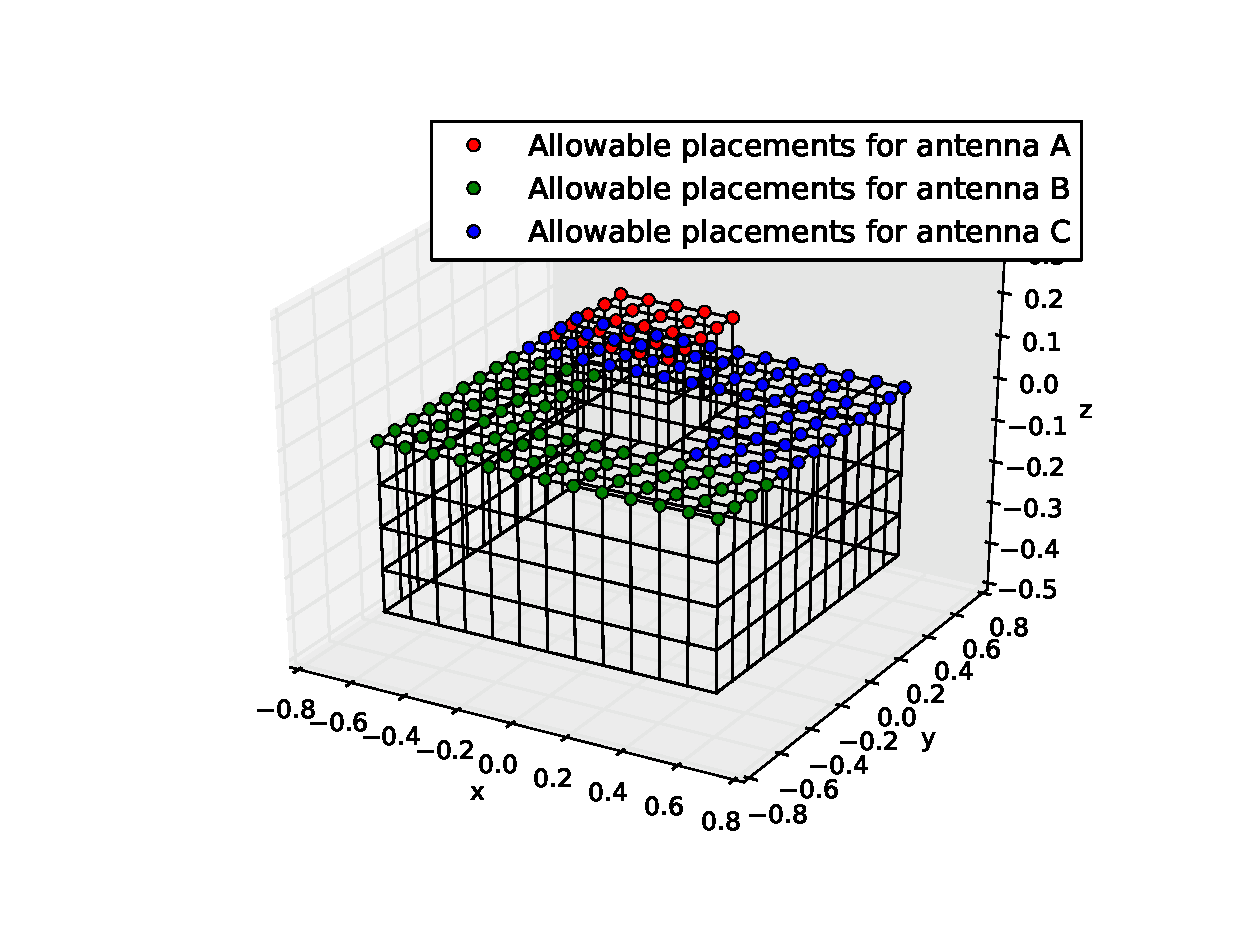
\includegraphics[width=\columnwidth,height=\columnwidth]{../paper/FIG/tc3_figure}%
            \caption*{\tiny Test Case \#3 with $126025 (71x71x25)$ allowable placements}%
        \end{subfigure}\hfill%
        \begin{subfigure}{.5\columnwidth}
            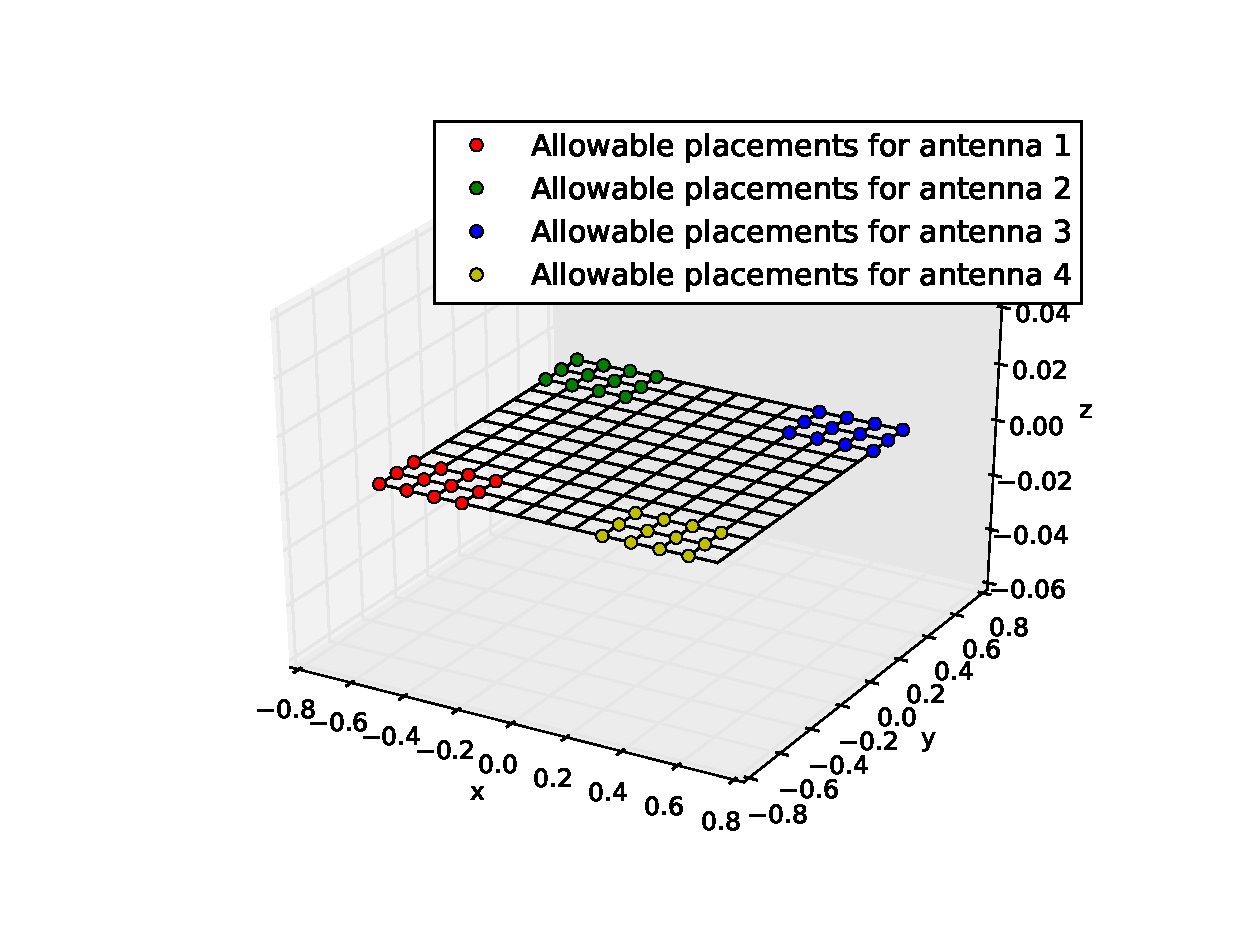
\includegraphics[width=\columnwidth, height=\columnwidth]{../paper/FIG/tc4_figure}%
            \caption*{\tiny Test Case \#4 with $20736 (12x12x12x12)$ allowable placements}%
        \end{subfigure}\hfill\\%
    \end{figure}
\end{frame}

\begin{frame}{Results - Test Case 1}
    \begin{figure}
        \vspace*{-0.35cm}
        \centering
        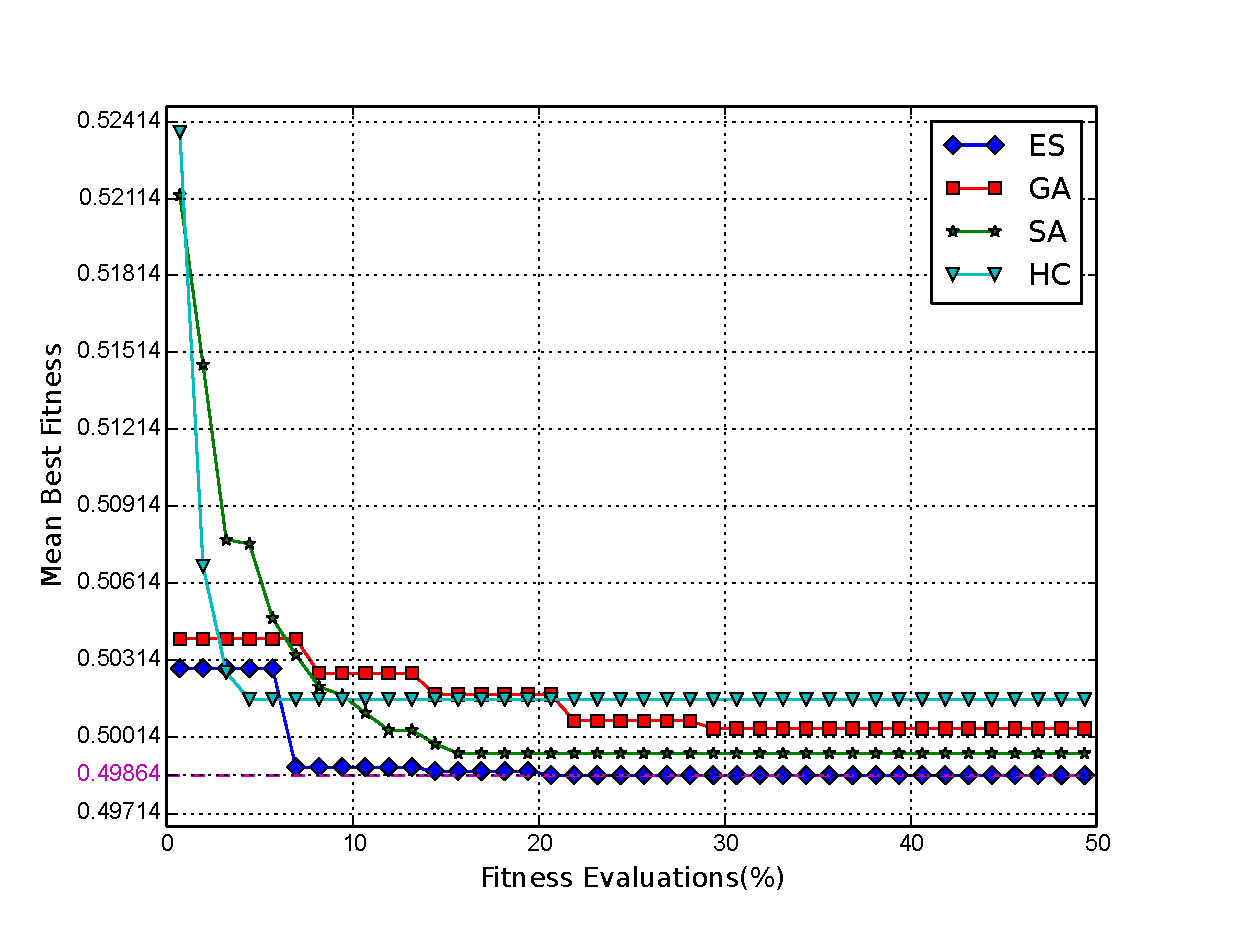
\includegraphics[scale=0.48]{../paper/FIG/tc1_mf}
    \end{figure}
\end{frame}

\begin{frame}{Results - Test Case 2}
    \begin{figure}
        \vspace*{-0.35cm}
        \centering
        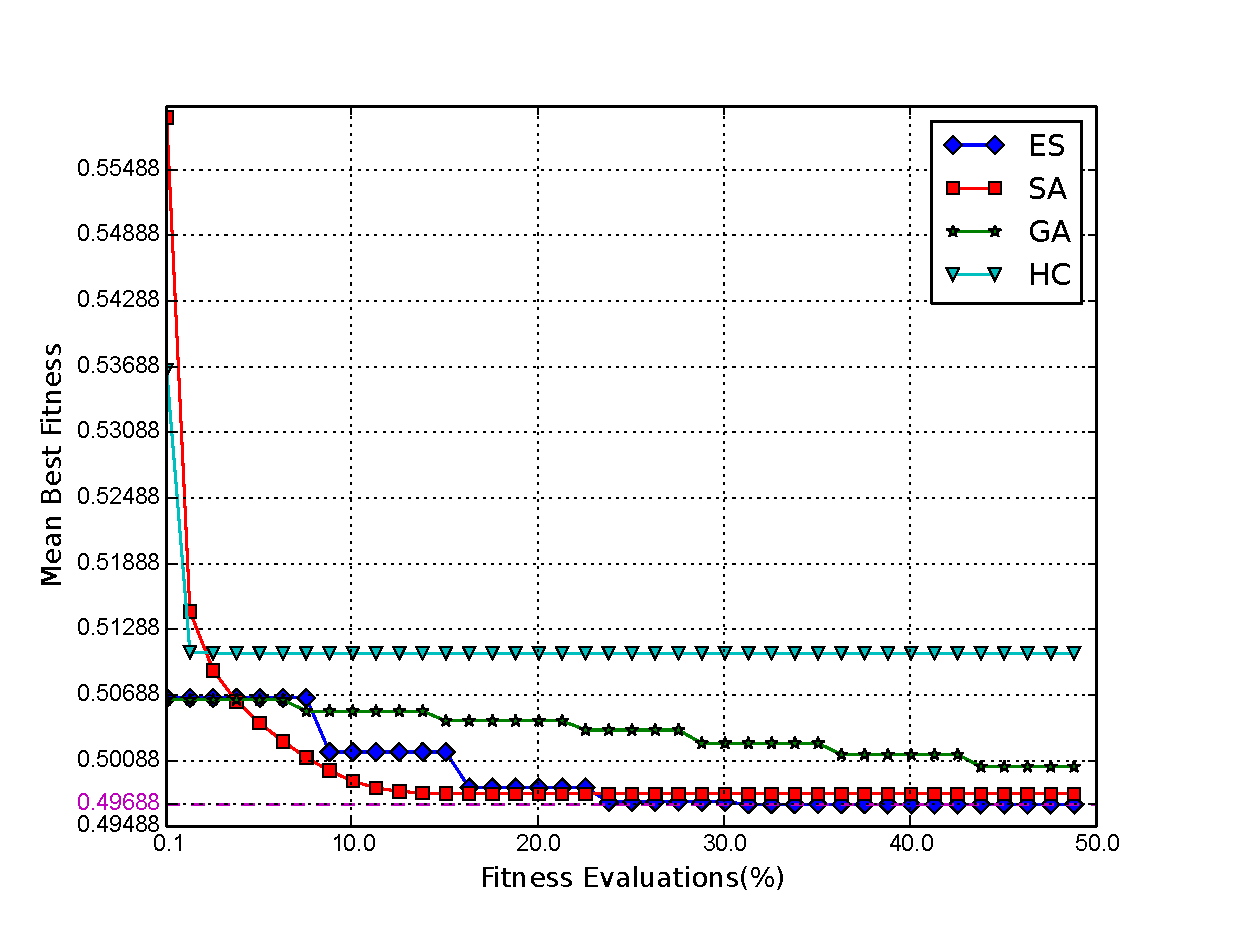
\includegraphics[scale=0.48]{../paper/FIG/tc2_mf}
    \end{figure}
\end{frame}


\begin{frame}{Results - Test Case 3}
    \begin{figure}
        \vspace*{-0.35cm}
        \centering
        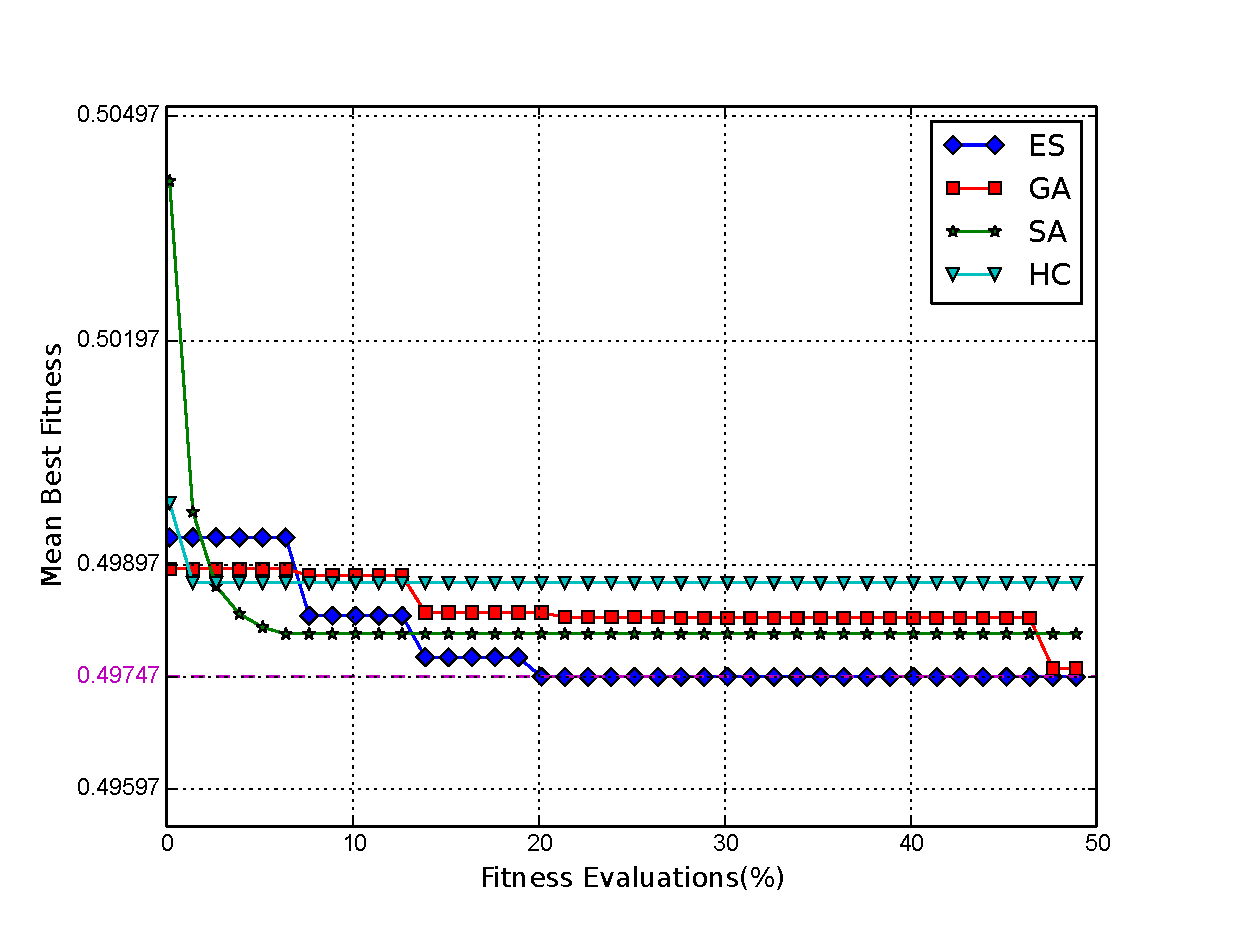
\includegraphics[scale=0.48]{../paper/FIG/tc3_mf}
    \end{figure}
\end{frame}


\begin{frame}{Results - Test Case 4}
    \begin{figure}
        \vspace*{-0.35cm}
        \centering
        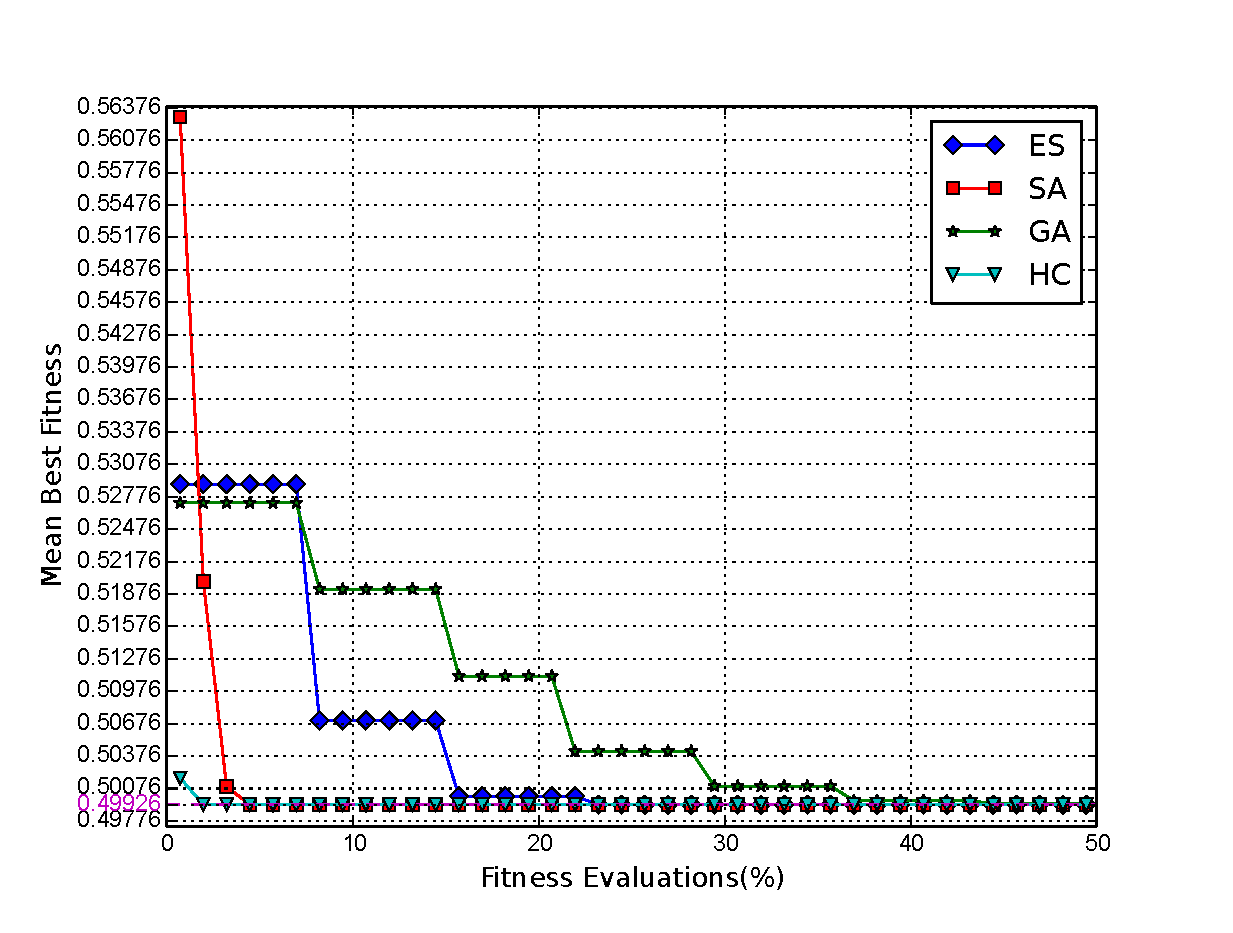
\includegraphics[scale=0.48]{../paper/FIG/tc4_mf}
    \end{figure}
\end{frame}


\begin{frame}{Results - Mean Best Fitness With Std. Dev.}
    \begin{figure}
        \vspace*{-0.35cm}
        \centering
        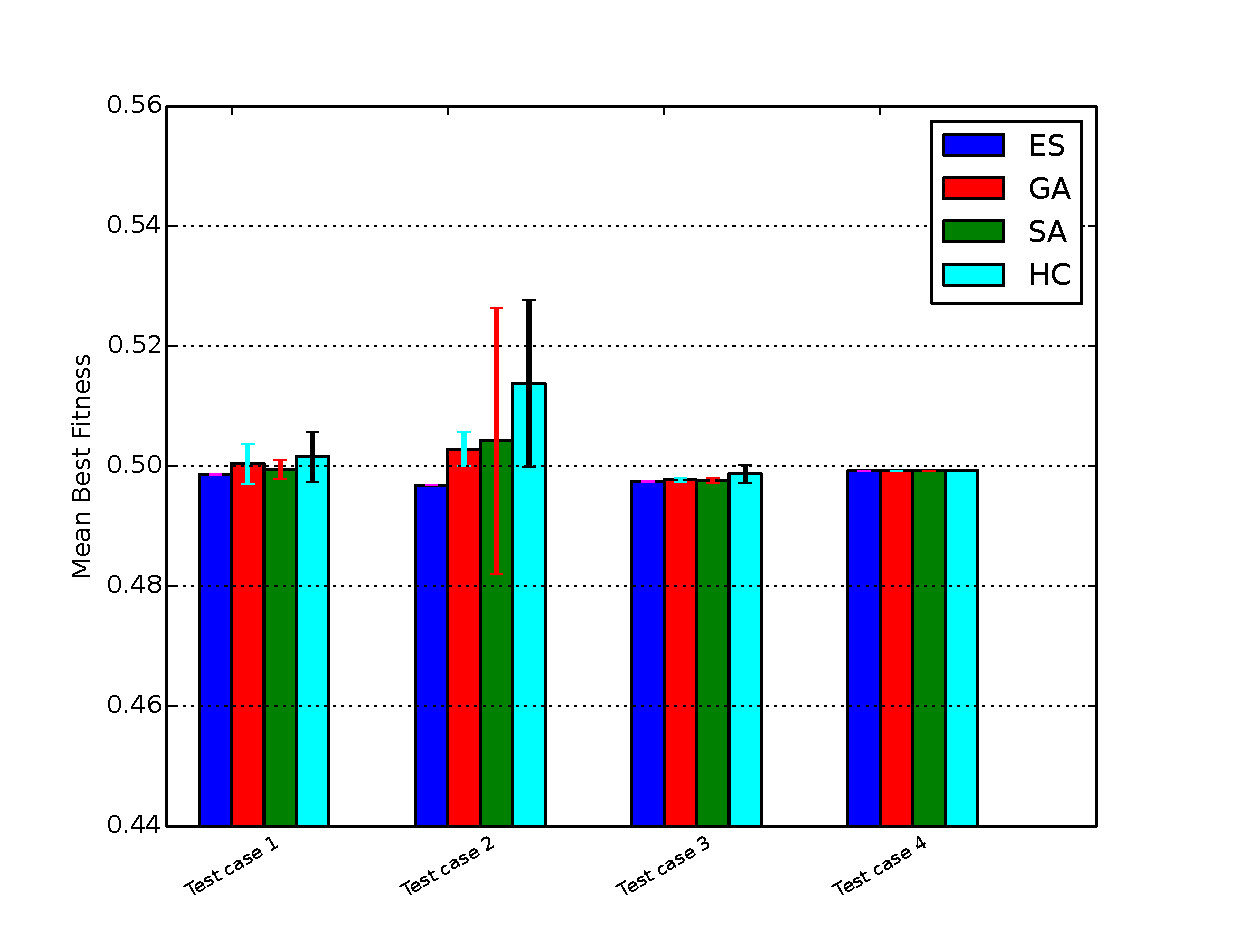
\includegraphics[scale=0.48]{../paper/FIG/tc_mfwerr}
    \end{figure}
\end{frame}

\begin{frame}{Results - Success Rates}
    \begin{figure}
        \vspace*{-0.35cm}
        \centering
        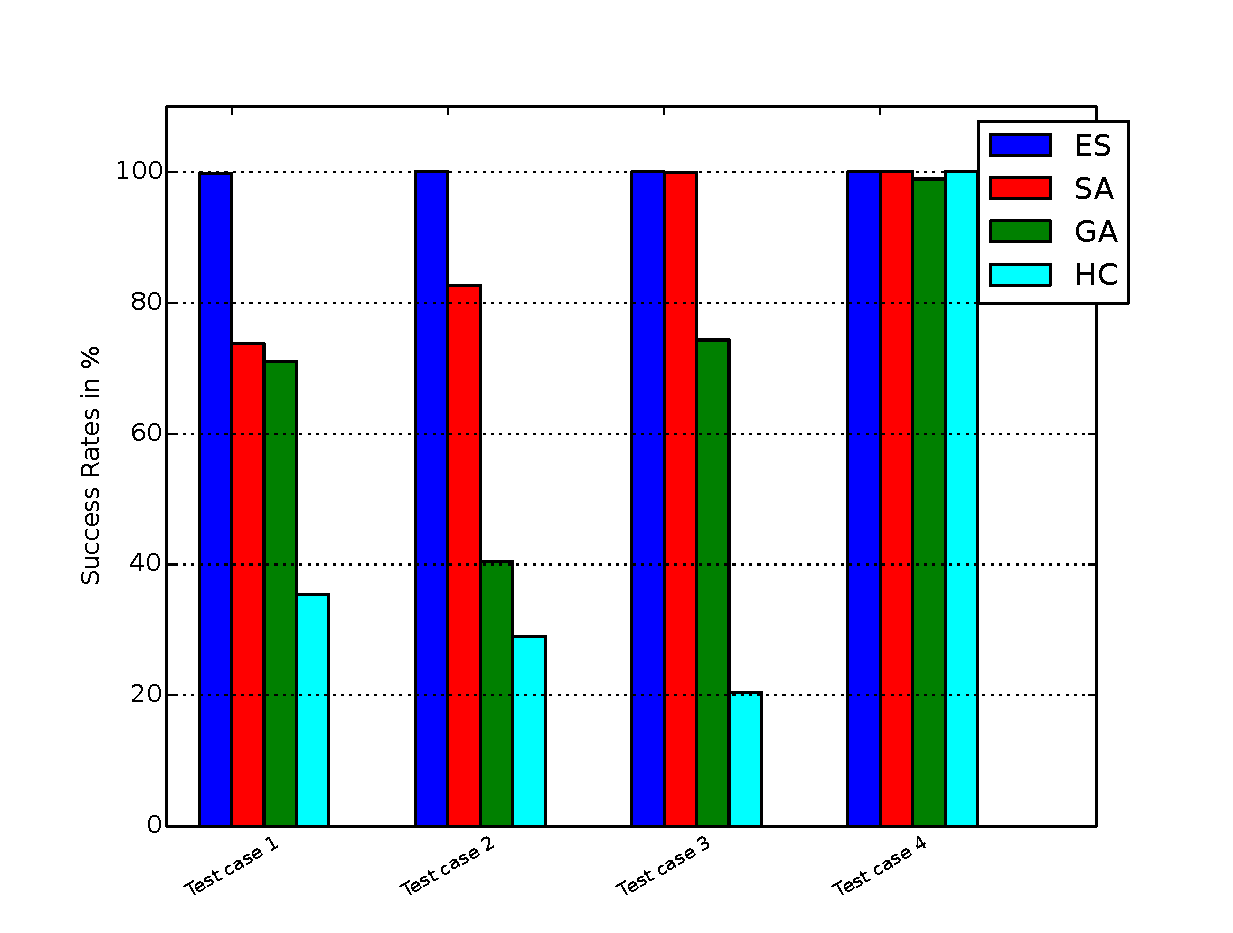
\includegraphics[scale=0.48]{../paper/FIG/tc_sp}
    \end{figure}
\end{frame}

\begin{frame}{Conclusion}
    \begin{itemize}
        \item Formulation of the antenna placement problem
        \item Generic problem formulation to accommodate multiple antennas and platforms
        \item Optimal placements found using stochastic algorithms
    \end{itemize}
\end{frame}

\end{document}
